\DocumentMetadata{%
 %  uncompress, %only for debugging!!
  pdfversion=2.0,
  testphase={phase-II, tabular, graphic}%
 % testphase={phase-II,math, tabular, graphic}% TOC Does not work
   % testphase={phase-III,math}% TOC works
}
\tagpdfsetup{activate, tabsorder=structure}
% Use the following to fix bug in November 2023 download of LaTeX
\ExplSyntaxOn
\cs_generate_variant:Nn\__tag_prop_gput:Nnn{cnx}
\ExplSyntaxOff
\documentclass[11pt,
  english,
  letterpaper,
]{article}
\usepackage{sa4ss}
\usepackage{amsmath,amssymb,array}
\usepackage{booktabs}

% From tagged-template.latex
\usepackage{lmodern}
\usepackage{ifxetex,ifluatex}
\ifnum 0\ifxetex 1\fi\ifluatex 1\fi=0 % if pdftex
  \usepackage[T1]{fontenc}
  \usepackage[utf8]{inputenc}
  \usepackage{textcomp} % provide euro and other symbols
\else % if luatex or xetex
  \usepackage{unicode-math}
  \defaultfontfeatures{Scale=MatchLowercase}
  \defaultfontfeatures[\rmfamily]{Ligatures=TeX,Scale=1}
\fi

% Use upquote if available, for straight quotes in verbatim environments
\IfFileExists{upquote.sty}{\usepackage{upquote}}{}
\IfFileExists{microtype.sty}{% use microtype if available
  \usepackage[]{microtype}
  \UseMicrotypeSet[protrusion]{basicmath} % disable protrusion for tt fonts
}{}
\makeatletter
\@ifundefined{KOMAClassName}{% if non-KOMA class
  \IfFileExists{parskip.sty}{%
    \usepackage{parskip}
  }{% else
    \setlength{\parindent}{0pt}
    \setlength{\parskip}{6pt plus 2pt minus 1pt}}
}{% if KOMA class
  \KOMAoptions{parskip=half}}
\makeatother
\usepackage{xcolor}
\IfFileExists{xurl.sty}{\usepackage{xurl}}{} % add URL line breaks if available
\hypersetup{
  pdftitle={Status of copper rockfish (Sebastes caurinus) along the California South of Pt. Conception U.S. West coast in 2023},
  pdflang={en},
  hidelinks,
  pdfcreator={LaTeX via pandoc}}
\urlstyle{same} % disable monospaced font for URLs
\usepackage{longtable}
% Correct order of tables after \paragraph or \subparagraph
\usepackage{etoolbox}
\makeatletter
\patchcmd\longtable{\par}{\if@noskipsec\mbox{}\fi\par}{}{}
\makeatother
% Allow footnotes in longtable head/foot
\IfFileExists{footnotehyper.sty}{\usepackage{footnotehyper}}{\usepackage{footnote}}
\makesavenoteenv{longtable}
\usepackage{graphicx}
\makeatletter
\def\maxwidth{\ifdim\Gin@nat@width>\linewidth\linewidth\else\Gin@nat@width\fi}
\def\maxheight{\ifdim\Gin@nat@height>\textheight\textheight\else\Gin@nat@height\fi}
\makeatother
% Scale images if necessary, so that they will not overflow the page
% margins by default, and it is still possible to overwrite the defaults
% using explicit options in \includegraphics[width, height, ...]{}
\setkeys{Gin}{width=\maxwidth,height=\maxheight,keepaspectratio}
% Set default figure placement to htbp
\makeatletter
\def\fps@figure{htbp}
\makeatother
\setlength{\emergencystretch}{3em} % prevent overfull lines
\providecommand{\tightlist}{%
  \setlength{\itemsep}{0pt}\setlength{\parskip}{0pt}}
\setcounter{secnumdepth}{5}
\ifxetex
  % Load polyglossia as late as possible: uses bidi with RTL langages (e.g. Hebrew, Arabic)
  \usepackage{polyglossia}
  \setmainlanguage[]{}
\else
  \usepackage[shorthands=off,main=english]{babel}
\fi

%Define cslreferences environment, required by pandoc 2.8
%https://github.com/rstudio/rmarkdown/issues/1649
\newlength{\csllabelwidth}
\setlength{\csllabelwidth}{3em}
\newlength{\cslhangindent}
\setlength{\cslhangindent}{1.5em}
% for Pandoc 2.8 to 2.10.1
\newenvironment{cslreferences}%
  {}%
  {\par}
% For Pandoc 2.11+
\newenvironment{CSLReferences}[2] % #1 hanging-ident, #2 entry spacing
 {% don't indent paragraphs
  \setlength{\parindent}{0pt}
  % turn on hanging indent if param 1 is 1
  \ifodd #1 \everypar{\setlength{\hangindent}{\cslhangindent}}\ignorespaces\fi
  % set entry spacing
  \ifnum #2 > 0
  \setlength{\parskip}{#2\baselineskip}
  \fi
 }%
 {}
\usepackage{calc}  % for \widthof, \maxof in minipage
\newcommand{\CSLBlock}[1]{#1\hfill\break}
\newcommand{\CSLLeftMargin}[1]{\parbox[t]{\csllabelwidth}{#1}}
\newcommand{\CSLRightInline}[1]{\parbox[t]{\linewidth - \csllabelwidth}{#1}\break}
\newcommand{\CSLIndent}[1]{\hspace{\cslhangindent}#1}


\providecommand{\tightlist}{%
  \setlength{\itemsep}{0pt}\setlength{\parskip}{0pt}}


\date{}
\newcommand{\trTitle}{Status of copper rockfish (\emph{Sebastes caurinus}) along the California South of Pt. Conception U.S. West coast in 2023}
\newcommand{\trYear}{2023}
\newcommand{\trMonth}{March}
\newcommand{\trAuthsLong}{truetruetrue}
\newcommand{\trAuthsBack}{Wetzel, C.R., M.H. Monk, J. Coates}
\newcommand{\trCitation}{
\begin{hangparas}{1em}{1}
\trAuthsBack{}. \trYear{}. \trTitle{}. \glsentrylong{pfmc}, Portland, Oregon. \pageref{LastPage}{}\,p.
\end{hangparas}}

\begin{document}

%%%%% Frontmatter %%%%%

% Footnote symbols in front matter
\renewcommand*{\thefootnote}{\fnsymbol{footnote}}

\small
\thispagestyle{empty}
\pagenumbering{roman}
\noindent
\begin{center}
\title{Status of copper rockfish (\emph{Sebastes caurinus}) along the California South of Pt. Conception U.S. West coast in 2023}
% \textnormal{\MakeTextUppercase{\trTitle{}}}
\vspace{1.5cm}
{\Large\textbf\newline{Status of copper rockfish (\emph{Sebastes caurinus}) along the California South of Pt. Conception U.S. West coast in 2023}}
\vfill
by\\
Chantel R. Wetzel\textsuperscript{1}\\
Melissa H. Monk\textsuperscript{2}\\
Julia Coates\textsuperscript{3}\vfill
\textsuperscript{1}Northwest Fisheries Science Center, U.S. Department of Commerce, National Oceanic and Atmospheric Administration, National Marine Fisheries Service, 2725 Montlake Boulevard East, Seattle, Washington 98112\\
\textsuperscript{2}Southwest Fisheries Science Center, U.S. Department of Commerce, National Oceanic and Atmospheric Administration, National Marine Fisheries Service, 110 McAllister Way, Santa Cruz, California 95060\\
\textsuperscript{3}.na.character\vfill
\trMonth{} \trYear{}
\end{center}
\clearpage

% Fourth page: Colophon
\thispagestyle{empty}
\vspace*{\fill}
\begin{center}
\copyright{} \glsentrylong{pfmc}, \trYear{}\\
\end{center}
\par
\bigskip
\noindent
Correct citation for this publication:
\bigskip
\par
\trCitation{}
\clearpage

% Add TOC to pdf bookmarks (clickable pdf)
\pdfbookmark[1]{\contentsname}{toc}

% Table of contents page, lists of figures and tables
\tableofcontents\clearpage
\label{TRlastRoman}
\clearpage

% Table of contents
\newpage
\thispagestyle{empty} % to remove page number

% Settings for the main document
\pagenumbering{arabic}  % Regular page numbers
\pagestyle{plain}  % No page number on first page of main document, use 'empty'
\renewcommand*{\thefootnote}{\arabic{footnote}}  % Back to numeric footnotes
\setcounter{footnote}{0}  % And start at 1
\renewcommand{\headrulewidth}{0.5pt}
\renewcommand{\footrulewidth}{0.5pt}
%\pagestyle{fancy}\fancyhead[c]{Draft: Do not cite or circulate}

\newcommand{\lt}{\ensuremath <}
\newcommand{\gt}{\ensuremath >}

\pagebreak
\pagenumbering{roman}
\setcounter{page}{1}

\renewcommand{\thetable}{\roman{table}}
\renewcommand{\thefigure}{\roman{figure}}

\setlength\parskip{0.5em plus 0.1em minus 0.2em}

\hypertarget{executive-summary}{%
\section*{Executive summary}\label{executive-summary}}
\addcontentsline{toc}{section}{Executive summary}

\hypertarget{stock}{%
\subsection*{Stock}\label{stock}}
\addcontentsline{toc}{subsection}{Stock}

This assessment reports the status of copper rockfish (\emph{Sebastes caurinus}) off the California South of Pt. Conception U.S. West coast using data through 2022.

\hypertarget{catches}{%
\subsection*{Catches}\label{catches}}
\addcontentsline{toc}{subsection}{Catches}

Replace text with trends and current levels. Include Table for last 10 years. Include Figure with long-term estimates.

\begingroup\fontsize{10}{12}\selectfont
\begingroup\fontsize{10}{12}\selectfont

\begin{longtable}[t]{r>{\centering\arraybackslash}p{2cm}>{\centering\arraybackslash}p{2cm}>{\centering\arraybackslash}p{2cm}}
\caption{\label{tab:removalsES}Recent landings by fleet and total landings summed across fleets.}\\
\toprule
Year & CA N Commercial & CA N Recreational & Total Landings\\
\midrule
\endfirsthead
\caption[]{Recent landings by fleet and total landings summed across fleets. \textit{(continued)}}\\
\toprule
Year & CA N Commercial & CA N Recreational & Total Landings\\
\midrule
\endhead

\endfoot
\bottomrule
\endlastfoot
2011 & 2.45 & 23.43 & 25.88\\
2012 & 3.19 & 31.69 & 34.88\\
2013 & 2.94 & 22.83 & 25.77\\
2014 & 3.26 & 33.73 & 36.99\\
2015 & 3.65 & 62.00 & 65.65\\
2016 & 3.44 & 62.92 & 66.36\\
2017 & 6.07 & 132.61 & 138.68\\
2018 & 9.87 & 92.98 & 102.85\\
2019 & 12.48 & 92.54 & 105.02\\
2020 & 14.63 & 51.58 & 66.21\\*
\end{longtable}
\endgroup{}
\endgroup{}


\begin{figure}
\centering
\includegraphics[width=1\textwidth,height=1\textheight]{N:/Assessments/CurrentAssessments/copper_rockfish_2023/models/sca/_bridging/2.4_dw/plots/catch2 landings stacked.png}
\caption{Landings by fleet used in the base model where catches in metric tons by fleet are stacked.\label{fig:es-catch}}
\end{figure}

\hypertarget{data-and-assessment}{%
\subsection*{Data and assessment}\label{data-and-assessment}}
\addcontentsline{toc}{subsection}{Data and assessment}

This assessment uses the stock assessment framework Stock Synthesis

\begin{verbatim}
[1] "3.30.20.00"
\end{verbatim}

(SS3).

Replace text with date of last assessment, type of assessment model, data available, new information, and information lacking.

\hypertarget{stock-biomass-and-dynamics}{%
\subsection*{Stock biomass and dynamics}\label{stock-biomass-and-dynamics}}
\addcontentsline{toc}{subsection}{Stock biomass and dynamics}

Replace text with trends and current levels relative to virgin or historic levels and description of uncertainty. Include Table for last 10 years. Include Figure with long-term estimates.

\begingroup\fontsize{10}{12}\selectfont
\begingroup\fontsize{10}{12}\selectfont

\begin{longtable}[t]{r>{\centering\arraybackslash}p{1.57cm}>{\centering\arraybackslash}p{1.57cm}>{\centering\arraybackslash}p{1.57cm}>{\centering\arraybackslash}p{1.57cm}>{\centering\arraybackslash}p{1.57cm}>{\centering\arraybackslash}p{1.57cm}}
\caption{\label{tab:ssbES}Estimated recent trend in spawning output and the fraction unfished and the 95 percent intervals.}\\
\toprule
Year & Spawning Output & Lower Interval & Upper Interval & Fraction Unfished & Lower Interval & Upper Interval\\
\midrule
\endfirsthead
\caption[]{Estimated recent trend in spawning output and the fraction unfished and the 95 percent intervals. \textit{(continued)}}\\
\toprule
Year & Spawning Output & Lower Interval & Upper Interval & Fraction Unfished & Lower Interval & Upper Interval\\
\midrule
\endhead

\endfoot
\bottomrule
\endlastfoot
2011 & 61.25 & 36.39 & 86.11 & 0.26 & 0.17 & 0.35\\
2012 & 63.22 & 37.66 & 88.79 & 0.27 & 0.18 & 0.37\\
2013 & 64.35 & 38.20 & 90.50 & 0.28 & 0.18 & 0.37\\
2014 & 62.52 & 35.95 & 89.09 & 0.27 & 0.17 & 0.37\\
2015 & 61.70 & 34.79 & 88.62 & 0.26 & 0.16 & 0.37\\
2016 & 58.89 & 31.79 & 85.99 & 0.25 & 0.15 & 0.35\\
2017 & 54.21 & 27.04 & 81.38 & 0.23 & 0.13 & 0.34\\
2018 & 50.17 & 22.94 & 77.40 & 0.22 & 0.11 & 0.32\\
2019 & 44.70 & 17.48 & 71.91 & 0.19 & 0.09 & 0.30\\
2020 & 40.81 & 13.49 & 68.13 & 0.18 & 0.07 & 0.28\\
2021 & 42.28 & 14.46 & 70.10 & 0.18 & 0.07 & 0.29\\*
\end{longtable}
\endgroup{}
\endgroup{}


\begin{figure}
\centering
\includegraphics[width=1\textwidth,height=1\textheight]{N:/Assessments/CurrentAssessments/copper_rockfish_2023/models/sca/_bridging/2.4_dw/plots/ts7_Spawning_output_with_95_asymptotic_intervals_intervals.png}
\caption{Estimated time series of spawning output (circles and line: median; light broken lines: 95 percent intervals) for the base model.\label{fig:es-sb}}
\end{figure}

\begin{figure}
\centering
\includegraphics[width=1\textwidth,height=1\textheight]{N:/Assessments/CurrentAssessments/copper_rockfish_2023/models/sca/_bridging/2.4_dw/plots/ts9_Relative_spawning_output_intervals.png}
\caption{Estimated time series of fraction of unfished spawning output (circles and line: median; light broken lines: 95 percent intervals) for the base model.\label{fig:es-depl}}
\end{figure}

\clearpage

\hypertarget{recruitment}{%
\subsection*{Recruitment}\label{recruitment}}
\addcontentsline{toc}{subsection}{Recruitment}

Replace text with trends and current levels relative to virgin or historic levels and description of uncertainty. Include Table for last 10 years. Include Figure with long-term estimates.

\begingroup\fontsize{10}{12}\selectfont
\begingroup\fontsize{10}{12}\selectfont

\begin{longtable}[t]{r>{\centering\arraybackslash}p{1.57cm}>{\centering\arraybackslash}p{1.57cm}>{\centering\arraybackslash}p{1.57cm}>{\centering\arraybackslash}p{1.57cm}>{\centering\arraybackslash}p{1.57cm}>{\centering\arraybackslash}p{1.57cm}}
\caption{\label{tab:recrES}Estimated recent trend in recruitment and recruitment deviations and the 95 percent intervals.}\\
\toprule
Year & Recruitment & Lower Interval & Upper Interval & Recruitment Deviations & Lower Interval & Upper Interval\\
\midrule
\endfirsthead
\caption[]{Estimated recent trend in recruitment and recruitment deviations and the 95 percent intervals. \textit{(continued)}}\\
\toprule
Year & Recruitment & Lower Interval & Upper Interval & Recruitment Deviations & Lower Interval & Upper Interval\\
\midrule
\endhead

\endfoot
\bottomrule
\endlastfoot
2011 & 208.08 & 88.19 & 490.98 & -0.08 & -0.92 & 0.76\\
2012 & 375.56 & 193.20 & 730.05 & 0.47 & -0.10 & 1.03\\
2013 & 450.80 & 238.05 & 853.71 & 0.59 & 0.07 & 1.11\\
2014 & 339.33 & 167.62 & 686.93 & 0.22 & -0.39 & 0.84\\
2015 & 302.70 & 144.89 & 632.40 & 0.04 & -0.60 & 0.69\\
2016 & 274.43 & 125.94 & 597.99 & -0.10 & -0.80 & 0.61\\
2017 & 228.86 & 94.64 & 553.46 & -0.31 & -1.17 & 0.55\\
2018 & 308.42 & 107.18 & 887.47 & -0.13 & -1.23 & 0.97\\
2019 & 356.42 & 117.43 & 1081.76 & 0.00 & -1.18 & 1.18\\
2020 & 358.34 & 117.95 & 1088.65 & 0.00 & -1.18 & 1.18\\
2021 & 360.74 & 118.70 & 1096.32 & 0.00 & -1.18 & 1.18\\*
\end{longtable}
\endgroup{}
\endgroup{}


\begin{figure}
\centering
\includegraphics[width=1\textwidth,height=1\textheight]{N:/Assessments/CurrentAssessments/copper_rockfish_2023/models/sca/_bridging/2.4_dw/plots/ts11_Age-0_recruits_(1000s)_with_95_asymptotic_intervals.png}
\caption{Estimated time series of age-0 recruits (1000s) for the base model with 95 percent intervals.\label{fig:es-recruits}}
\end{figure}

\clearpage

\hypertarget{exploitation-status}{%
\subsection*{Exploitation status}\label{exploitation-status}}
\addcontentsline{toc}{subsection}{Exploitation status}

Replace text with total catch divided by exploitable biomass or SPR harvest rate. Include Table for last 10 years. Include Figure with trend in f relative to target vs.~trend in biomass relative to the target.

\begingroup\fontsize{10}{12}\selectfont
\begingroup\fontsize{10}{12}\selectfont

\begin{longtable}[t]{r>{\centering\arraybackslash}p{1.57cm}>{\centering\arraybackslash}p{1.57cm}>{\centering\arraybackslash}p{1.57cm}>{\centering\arraybackslash}p{1.57cm}>{\centering\arraybackslash}p{1.57cm}>{\centering\arraybackslash}p{1.57cm}}
\caption{\label{tab:exploitES}Estimated recent trend in the 1-SPR where SPR is the spawning potential ratio the exploitation rate, and the  95 percent intervals.}\\
\toprule
Year & 1-SPR & Lower Interval & Upper Interval & Exploitation Rate & Lower Interval & Upper Interval\\
\midrule
\endfirsthead
\caption[]{Estimated recent trend in the 1-SPR where SPR is the spawning potential ratio the exploitation rate, and the  95 percent intervals. \textit{(continued)}}\\
\toprule
Year & 1-SPR & Lower Interval & Upper Interval & Exploitation Rate & Lower Interval & Upper Interval\\
\midrule
\endhead

\endfoot
\bottomrule
\endlastfoot
2011 & 0.57 & 0.48 & 0.67 & 0.06 & 0.04 & 0.09\\
2012 & 0.62 & 0.52 & 0.71 & 0.07 & 0.05 & 0.10\\
2013 & 0.77 & 0.69 & 0.86 & 0.11 & 0.07 & 0.15\\
2014 & 0.71 & 0.61 & 0.80 & 0.09 & 0.05 & 0.12\\
2015 & 0.80 & 0.72 & 0.89 & 0.12 & 0.07 & 0.17\\
2016 & 0.87 & 0.80 & 0.95 & 0.15 & 0.09 & 0.21\\
2017 & 0.86 & 0.78 & 0.95 & 0.14 & 0.08 & 0.21\\
2018 & 0.91 & 0.84 & 0.98 & 0.18 & 0.09 & 0.27\\
2019 & 0.89 & 0.79 & 0.98 & 0.16 & 0.07 & 0.25\\
2020 & 0.44 & 0.28 & 0.60 & 0.04 & 0.02 & 0.07\\*
\end{longtable}
\endgroup{}
\endgroup{}


\begin{figure}
\centering
\includegraphics[width=1\textwidth,height=1\textheight]{N:/Assessments/CurrentAssessments/copper_rockfish_2023/models/sca/_bridging/2.4_dw/plots/SPR2_minusSPRseries.png}
\caption{Estimated 1 - relative spawning ratio (SPR) by year for the base model. The management target is plotted as a red horizontal line and values above this reflect harvest in excess of the proxy harvest rate.\label{fig:es-1-spr}}
\end{figure}

\hypertarget{ecosystem-considerations}{%
\subsection*{Ecosystem considerations}\label{ecosystem-considerations}}
\addcontentsline{toc}{subsection}{Ecosystem considerations}

shared text

\hypertarget{reference-points}\), i.e., the \(B_{MSY}\) proxy and the equilibrium stock size that results from fishing at the default harvest rate, i.e., the \(F_{MSY}\) proxy. Include Table of estimated reference points for ssb, SPR, exploitation rate, and yield based on SSB proxy for MSY, SPR proxy for MSY, and estimated MSY values.

\begingroup\fontsize{10}{12}\selectfont
\begingroup\fontsize{10}{12}\selectfont

\begin{longtable}[t]{r>{\centering\arraybackslash}p{2cm}>{\centering\arraybackslash}p{2cm}>{\centering\arraybackslash}p{2cm}}
\caption{\label{tab:referenceES}Summary of reference points and management quantities, including estimates of the  95 percent intervals.}\\
\toprule
 & Estimate & Lower Interval & Upper Interval\\
\midrule
\endfirsthead
\caption[]{Summary of reference points and management quantities, including estimates of the  95 percent intervals. \textit{(continued)}}\\
\toprule
 & Estimate & Lower Interval & Upper Interval\\
\midrule
\endhead

\endfoot
\bottomrule
\endlastfoot
Unfished Spawning Output & 233.04 & 216.73 & 249.35\\
Unfished Age 3+ Biomass (mt) & 2294.94 & 2134.31 & 2455.57\\
Unfished Recruitment (R0) & 243.71 & 226.65 & 260.76\\
Spawning Output (2021) & 42.28 & 14.46 & 70.10\\
Fraction Unfished (2021) & 0.18 & 0.07 & 0.29\\
Reference Points Based SB40\textbackslash{}\% & NA & NA & NA\\
Proxy Spawning Output SB40\textbackslash{}\% & 93.22 & 86.69 & 99.74\\
SPR Resulting in SB40\textbackslash{}\% & 0.46 & 0.46 & 0.46\\
Exploitation Rate Resulting in SB40\textbackslash{}\% & 0.05 & 0.05 & 0.06\\
Yield with SPR Based On SB40\textbackslash{}\% (mt) & 54.40 & 52.78 & 56.01\\
Reference Points Based on SPR Proxy for MSY & NA & NA & NA\\
Proxy Spawning Output (SPR50) & 103.97 & 96.69 & 111.25\\
SPR50 & 0.50 & NA & NA\\
Exploitation Rate Corresponding to SPR50 & 0.05 & 0.04 & 0.05\\
Yield with SPR50 at SB SPR (mt) & 51.84 & 50.31 & 53.38\\
Reference Points Based on Estimated MSY Values & NA & NA & NA\\
Spawning Output at MSY (SB MSY) & 62.60 & 58.44 & 66.77\\
SPR MSY & 0.34 & 0.34 & 0.34\\
Exploitation Rate Corresponding to SPR MSY & 0.08 & 0.08 & 0.09\\
MSY (mt) & 58.08 & 56.31 & 59.84\\*
\end{longtable}
\endgroup{}
\endgroup{}


\begin{figure}
\centering
\includegraphics[width=1\textwidth,height=1\textheight]{N:/Assessments/CurrentAssessments/copper_rockfish_2023/models/sca/_bridging/2.4_dw/plots/SPR4_phase.png}
\caption{Phase plot of estimated 1-SPR versus fraction unfished for the base model.\label{fig:es-phase}}
\end{figure}

\begin{figure}
\centering
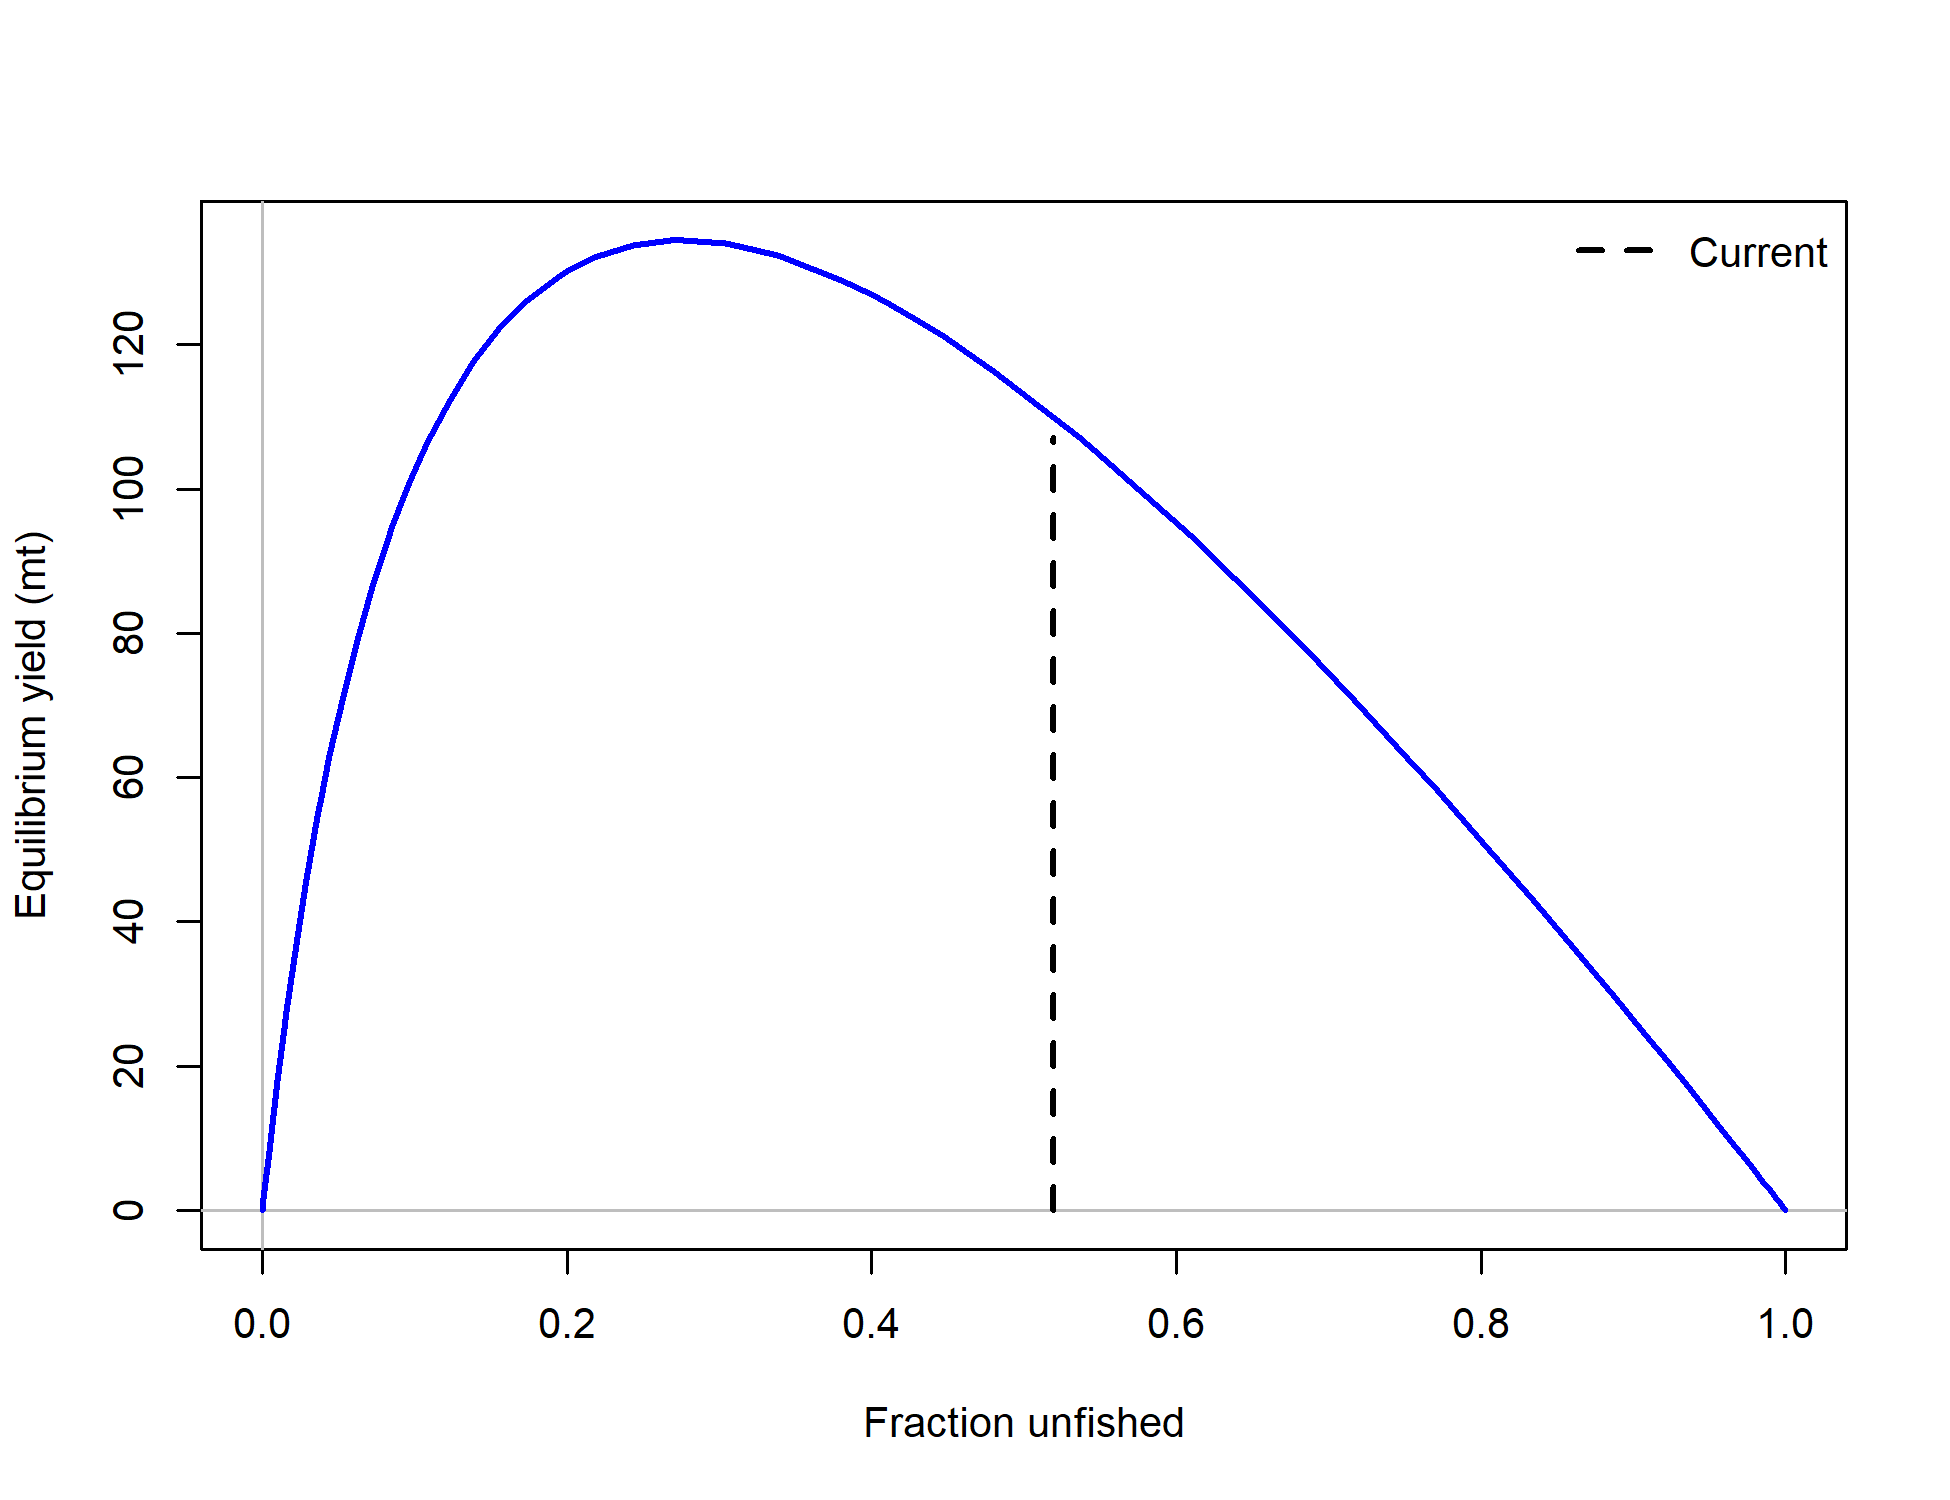
\includegraphics[width=1\textwidth,height=1\textheight]{N:/Assessments/CurrentAssessments/copper_rockfish_2023/models/sca/_bridging/2.4_dw/plots/yield2_yield_curve_with_refpoints.png}
\caption{Equilibrium yield curve for the base case model. Values are based on the 2020 fishery selectivities and with steepness fixed at 0.80.\label{fig:es-yield}}
\end{figure}

\hypertarget{management-performance}{%
\subsection*{Management performance}\label{management-performance}}
\addcontentsline{toc}{subsection}{Management performance}

Include Table of most recent 10 years of catches in comparison with OFL, ABC, HG, and OY/ACL values, overfishing levels, actual catch and discard. Include OFL (encountered), OFL (retained), and OFL (dead) if different due to discard and discard mortality.

\hypertarget{unresolved-problems-and-major-uncertainties}{%
\subsection*{Unresolved problems and major uncertainties}\label{unresolved-problems-and-major-uncertainties}}
\addcontentsline{toc}{subsection}{Unresolved problems and major uncertainties}

shared text

\hypertarget{decision-table-and-projections}{%
\subsection*{Decision table and projections}\label{decision-table-and-projections}}
\addcontentsline{toc}{subsection}{Decision table and projections}

Replace text with projected yields (OFL, ABC, and ACL), spawning biomass, and stock depletion levels for each year. OFL calculations should be based on the assumption that future catches equal ABCs and not OFLs.

\hypertarget{scientific-uncertainty}{%
\subsection*{Scientific uncertainty}\label{scientific-uncertainty}}
\addcontentsline{toc}{subsection}{Scientific uncertainty}

The model estimated uncertainty around the 2023 spawning output was \(\sigma\) = 0.22 and the uncertainty around the OFL was \(\sigma\) = 0.15. This is likely an underestimate of overall uncertainty because of the necessity to fix several population dynamic parameters (e.g., steepness, recruitment variance, female natural mortality) and no explicit incorporation of model structural uncertainty (although see the decision table for alternative states of nature).

\hypertarget{research-and-data-needs}{%
\subsection*{Research and data needs}\label{research-and-data-needs}}
\addcontentsline{toc}{subsection}{Research and data needs}

shared text

\pagebreak
\setlength{\parskip}{5mm plus1mm minus1mm}
\pagenumbering{arabic}
\setcounter{page}{1}
\renewcommand{\thefigure}{\arabic{figure}}
\renewcommand{\thetable}{\arabic{table}}
\setcounter{table}{0}
\setcounter{figure}{0}

\hypertarget{introduction}{%
\section{Introduction}\label{introduction}}

\hypertarget{basic-information}{%
\subsection{Basic Information}\label{basic-information}}

This assessment reports the status of copper rockfish (\emph{Sebastes caurinus}) off the California coast, south of Point Conception, using data through 2022. This assessment does not account for populations located in Mexico waters and assumes that this southern population does not contribute to the population being assessed here.

\hypertarget{life-history}{%
\subsection{Life History}\label{life-history}}

Copper rockfish is a medium- to large-sized nearshore rockfish found from Mexico to Alaska. The core range is comparatively large, from northern Baja Mexico to the Gulf of Alaska, as well as in Puget Sound. Copper rockfish have historically been a part of both commercial and recreational fisheries throughout its range.

Copper rockfish are commonly found in waters less than 130 meters in depth in nearshore kelp forests and rocky habitat (Love 1996). The diets of copper rockfish consist primarily of crustaceans, mollusks, and fish (Lea, McAllister, and VenTresca 1999; Bizzarro, Yoklavich, and Wakefield 2017). The body coloring of copper rockfish varies across the West Coast with northern fish often exhibiting dark brown to olive with southern fish exhibiting yellow to olive-pink variations in color (D. J. Miller and Lea 1972), which initially led to them being designated as two separate species (\emph{S. caurinus} and \emph{S. vexillaris}).

Numerous genetic studies have been performed looking for genetic variation in copper rockfish, with variable outcomes. Genetic work has revealed significant differences between Puget Sound and coastal stocks (S. Dick, Shurin, and Taylor 2014). Stocks along the West Coast have not been determined to be genetically distinct populations, but significant population subdivision has been detected, indicating limited oceanographic exchange among geographically proximate locations (Buonaccorsi et al. 2002; Johansson et al. 2008). A specific study examining copper rockfish populations off the coast of Santa Barbara and Monterey California identified a genetic break between the north and south, with moderate differentiation (Sivasundar and Palumbi 2010).

Copper rockfish are a relatively long-lived rockfish, estimated to live at least 50 years (Love 1996). Copper rockfish was determined to have the highest vulnerability (V = 2.27) of any West Coast groundfish stock evaluated in a productivity susceptibility analysis (J. M. Cope et al. 2011). This analysis calculated species-specific vulnerability scores based on two dimensions: productivity characterized by the life history and susceptibility that characterized how the stock could be impacted by fisheries and other activities.

\hypertarget{ecosystem-considerations-1}{%
\subsection{Ecosystem Considerations}\label{ecosystem-considerations-1}}

This stock assessment does not explicitly incorporate trophic interactions, habitat factors (other than as they inform relative abundance indices) or environmental factors into the assessment model, but a brief description of likely or potential ecosystem considerations are provided below.

As with most other rockfish and groundfish in the California Current, recruitment, or cohort (year-class) strength appears to be highly variable for the copper rockfish complex, with only a modest apparent relationship to estimated levels of spawning output. Oceanographic and ecosystem factors are widely recognized to be key drivers of recruitment variability for most species of groundfish, as well as most elements of California Current food webs. Empirical estimates of recruitment from pelagic juvenile rockfish surveys have been used to inform incoming year class strength for some of these stocks, however copper rockfish are infrequently encountered in these surveys. Between 1998 and 2013 the California Cooperative Oceanic Fisheries Investigation (CalCOFI) survey observed had 34 positive observations copper rockfish out of nearly 300,000 total juvenile \emph{Sebastes} encountered in juvenile surveys. (\textbf{thompson\_larval\_2017?})

\hypertarget{historical-and-current-fishery-information}{%
\subsection{Historical and Current Fishery Information}\label{historical-and-current-fishery-information}}

Off the coast of California south of Point Conception copper rockfish is caught in both commercial and recreational fisheries. Recreational removals have been the largest source of fishing mortality of copper rockfish across all years (Table \ref{tab:allcatches} and Figure \ref{fig:catch}). The recreational fishery is comprised of individual recreational fishers (Private/Rental, PR) and charter recreational private vessels (CPFV) which take groups of individuals out for day fishing trips. Across both types of recreational fishing the majority of effort occurs around rocky reefs that can be accessed via a day-trips.

The recreational fishery in the early part of the 20th century was focused on nearshore waters near ports, with expanded activity further from port and into deeper depths over time (R. R. Miller et al. 2014). Prior to the groundfish fishery being declared a federal disaster in 2000, and the subsequent rebuilding period, there were no time or area closures for groundfish. Access to deeper depths during this period spread effort over a larger area and filled bag limits with a greater diversity of species from both the shelf and nearshore. This resulted in lower catch of nearshore rockfish relative to the period after 2000 when 20 to 60 fm depth restrictions ranging from 20 fm in the Northern Management Area to 60 fm in the Southern Management Area were put in place in various management area delineations along the state (see Appendix Section \ref{ca-man}). This shifting effort onto the nearshore, concomitantly increased catch rates for nearshore rockfish including copper rockfish in the remaining open depths, though season lengths were greatly curtailed.

Following all previously overfished groundfish species, other than yelloweye rockfish, being declared rebuilt by 2019, deeper depth restrictions were offered in the Southern Management area allowing resumed access to shelf rockfish in less than 75 fm and are currently 100 fm as of 2021. The increased access to deeper depths south of Point Conception with the rebuilding of cowcod is expected to reduce the effort in nearshore waters where copper rockfish is most prevalent. To the north of Point Conception where yelloweye rockfish are prevalent, depth constraints persist and effort remains focused on the nearshore in 30 to 50 fm depending on the management area. As yelloweye rockfish continues to rebuild, incremental increases in access to deeper depths are expected, which will likely further reduce the effort in nearshore waters where copper rockfish is most prevalent.

Prior to development of the live fish market in the 1980s, there was very little commercial catch of copper rockfish, with dead copper rockfish fetching a low ex-vessel price per pound. Copper rockfish were targeted along with other rockfish to some degree in the nearshore or caught as incidental catch by vessels targeting other more valuable stocks such as lingcod. Most fish were caught using hook and line gear, though some were caught using traps, gill nets and, rarely, trawl gear. Trawling was prohibited within three miles of shore in 1953 and gill netting within three miles of shore was prohibited in 1994, preventing access to a high proportion of the species habitat with these gear types. Copper rockfish were caught along with other rockfish to some degree in the nearshore or caught as bycatch by vessels targeting other more valuable stocks such as lingcod.

In the late 1980s and early 1990s a market for fish landed live arose out of Los Angeles and the Bay area, driven by demand from Asian restaurants and markets. The growth of the live fish market was driven by consumers willing to pay a higher price for live fish, ideally plate-sized (12 - 14 inches or 30.5 - 35.6 cm). Live fish landed for the restaurant market are lumped into two categories, small (1 - 3 lbs.) or large (3 - 6 lbs.), with small, plate-sized, fish fetching higher prices at market ranging between \$5 -7 per fish (Bill James, personal communication). Copper rockfish is one of the many rockfish species that is included in the commercial live fish fishery. The proportion of copper rockfish being landed live vs.~dead since 2000 by California commercial fleets ranges between 50 to greater than 70 percent in the southern and northern areas, respectively.

With the development and expansion of the nearshore live fish fishery during the 1980s and 1990s, new entrants in this open access fishery were drawn by premium ex-vessel price per pound for live fish, resulting in over-capitalization of the fishery. Since 2002, the California Department of Fish and Wildlife (CDFW) has managed 19 nearshore species in accordance with Nearshore Fisheries Management Plan (Wilson-Vandenberg, Larinto, and Key 2014). In 2003, the CDFW implemented a Nearshore Restricted Access Permit system, including the requirement of a Deeper Nearshore Fishery Species Permit to retain copper rockfish, with the overall goal of reducing the number of participants to a more sustainable level, with permit issuance based on historical landings history by the retrospective qualifying date. The result was a reduction in permits issued from 1,127 in 1999 to 505 in 2003, greatly reducing catch levels. In addition, reduced trip limits, season closures in March and April and depth restrictions were implemented to address bycatch of overfished species and associated constraints from their low catch limits.

The population of copper rockfish south of Point Conception to the U.S./Mexico border is assessed here as a separate stock (Figure \ref{fig:map}). This decision was made based on oceanographic conditions and previous assessments of copper rockfish. The stock split in California waters at Point Conception accounts for water circulation patterns that create a natural barrier between nearshore rockfish population north and south of the area.

\hypertarget{summary-of-management-history-and-performance}{%
\subsection{Summary of Management History and Performance}\label{summary-of-management-history-and-performance}}

Copper rockfish is managed by the Pacific Fishery Management Council (PFMC) as a part of the Nearshore Rockfish North and Nearshore Rockfish South complexes, split at 40\(^\circ\) 10' N. lat. off the West Coast. Each complex, comprised of nearshore rockfish species, is managed based on a complex level overfishing limit (OFL) and annual catch limit (ACL) that are determined by summing the species-specific OFLs and ACLs (ACLs set equal to the Acceptable Biological Catches) contributions for all stocks managed in the complex (North or South). Removals for species within the Nearshore Rockfish North and South complexes are managed and tracked against the complex total OFL and ACL, rather than on a species by species basis.

\hypertarget{foreign-fisheries}{%
\subsection{Foreign Fisheries}\label{foreign-fisheries}}

Replace text.

\hypertarget{data}{%
\section{Data}\label{data}}

Data comprise the foundational components of stock assessment models. The decision to include or exclude particular data sources in an assessment model depends on many factors. These factors often include, but are not limited to, the way in which data were collected (e.g., measurement method and consistency); the spatial and temporal coverage of the data; the quantity of data available per desired sampling unit; the representativeness of the data to inform the modeled processes of importance; timing of when the data were provided; limitations imposed by the Terms of Reference; and the presence of an avenue for the inclusion of the data in the assessment model. Attributes associated with a data source can change through time, as can the applicability of the data source when different modeling approaches are explored (e.g., stock structure or time-varying processes). Therefore, the specific data sources included or excluded from this assessment should not necessarily constrain the selection of data sources applicable to future stock assessments for copper rockfish. Even if a data source is not directly used in the stock assessment they can provide valuable insights into biology, fishery behavior, or localized dynamics.

Data from a wide range of programs were available for possible inclusion in the current assessment model. Descriptions of each data source included in the model (Figure \ref{fig:data-plot}) and sources that were explored but not included in the base model are provided below. Data that were excluded from the base model were explicitly explored during the development of this stock assessment or have not changed since their past exploration in a previous copper rockfish stock assessment. In some cases, the inclusion of excluded data sources were explored through sensitivity analyses (see Section \ref{assessment-model}).

\hypertarget{fishery-dependent-data}{%
\subsection{Fishery-Dependent Data}\label{fishery-dependent-data}}

\hypertarget{commercial-fishery}{%
\subsubsection{Commercial Fishery}\label{commercial-fishery}}

\hypertarget{landings-and-discards}{%
\paragraph{Landings and Discards}\label{landings-and-discards}}

\hfill\break

Commercial landings prior to 1969 were extracted from the Southwest Fisheries Science Center (SWFSC) landings reconstruction database for estimates from the California Catch Reconstruction (Ralston et al. 2010). Landings in this database are divided into trawl, non-trawl, and unknown gear categories. Regions 7 and 8 as defined by Ralston et al. (2010) were assigned to south of Point Conception in California. Regions 2, 4, and 5 are associated with areas north of Point Conception. Region 6 in Ralston et al. (2010) included Santa Barbara County (mainly south of Point Conception), plus some major ports north of Point Conception. To allocate landings from Region 6 to the areas north and south of Point Conception, we followed an approach used by Dick et al. (2007) for the assessment of cowcod. Specifically, port-specific landings of total rockfish from the CDFW Fish Bulletin series were used to determine the annual fraction of landings in Region 6 that was north and south of Point Conception (Table \ref{tab:com-ratio}). Rockfish landings at that time were not reported at the species level. Although the use of total rockfish landings to partition landings in Region 6 is not ideal, we see this as the best available option in the absence of port-specific species composition data. Landings from unknown locations (Region 0) were allocated proportional to the landings from known regions.

In September 2005, the California Cooperative Groundfish Survey (CCGS) incorporated newly acquired commercial landings statistics from 1969-1980 into the CALCOM database (Pearson, Erwin, and Key 2008). The data consisted of landing receipts (``fish tickets''), including mixed species categories for rockfish. In order to assign rockfish landings to individual species, the earliest available species composition samples were applied to the fish ticket data by port, gear, and quarter. These `ratio estimator' landings are coded (internally) as market category 977 in the CALCOM database, and are used in this and past assessments as the best available landings for the time period 1969-1980 for all port complexes. See Appendix A of Dick et al. (2007) for further details.

Commercial fishery landings from 1981-2022 were extracted from the Pacific Fisheries Information Network (PacFIN) database (extracted February 6, 2023). Landings were separated north and south of Point Conception based on port of landing. Commercial landings for copper rockfish were split into two fleets based on the fish landed condition, live or dead, and aggregated across gear types (Table \ref{tab:allcatches} and Figure \ref{fig:catch}). The selection of this fleet structure was based on potential differences in selectivity by the fishery based on fish landed condition where the live fish fishery may be targeting fish of particular sizes (i.e., plate sized). The first year where fish were observed to be landed live for copper rockfish in the area south of Point Conception was 1994.

Discarding was not estimated within the model. The commercial catches, landings plus discards, were estimated external to the model based on data from the West Coast Groundfish Observer Program (WCGOP) data provided in the Groundfish Expanded Mortality Multiyear (GEMM) product. The GEMM provides expanded estimates of landings, discard, and catches based on observed trips by sector split north and south of 40\(^\circ\) 10' N. lat. for the commercial fishery. Estimated landings and discards south of 40\(^\circ\) 10' N. lat. from select sectors (LE Fixed Gear DTL - Hook and Line, Nearshore, CS - Hook and Line, OA Fixed Gear - Hook and Line, OA Fixed Gear - Pot, and LE Fixed Gear DTL - Pot) were used to calculate a discard rate (total discard divided by the sum of landings and discards by year) for 2002-2021. The annual discard rates were applied to the total landings by year to calculate catches for both areas south and north of Point Conception. The median discard rate south of 40\(^\circ\) 10' N. lat. from the select sectors between 2002-2021 in the GEMM was 3 percent. This discard rate was applied to landings between 1916-2001 and 2022 to determine catch by year. The assumptions around the discard rate by year had limited impact to the assumed total catches given the limited scale of removals by the commercial fishery for copper rockfish. Across all years, 1916-2022, the landings were increased by 2-3 percent by area (11 mt south of Point Conception and 26 mt north of Point Conception) to calculate the total catches.

\hypertarget{composition-data}{%
\paragraph{Composition Data}\label{composition-data}}

\hypertarget{recreational-fishery}{%
\subsubsection{Recreational Fishery}\label{recreational-fishery}}

\hypertarget{landings-and-discards-1}{%
\paragraph{Landings and Discards}\label{landings-and-discards-1}}

\hfill\break

The recreational fishery is the main source of exploitation of copper rockfish across California. The recreational catches of copper rockfish south of Point Conception in California waters peaked in the late 1970s and early 1980s. Catches declined in the 1990s and early 2000s (Table \ref{tab:allcatches} and Figure \ref{fig:catch}). The removals remained relatively low until 2015. Catches begun to increase in 2015, likely due to changes in harvest specifications (J. Cope et al. 2013). The catches decreased in 2020 due to COVID-19 impacts and remained relatively low in 2021 and 2022 due to reductions in the sub-bag limits in California for copper rockfish. The recreational fishery was split into two fleets based on fishing type (termed `modes'), a commercial passenger fishing vessel (CPFV, party/charter mode) fleet and a combined private or rental boats (PR mode) and shoreside (man-made and beach/bank modes) fleet. The catches associated with the shoreside mode for copper rockfish are limited and did not justify a separate fishing fleet within the model.

Recreational landing estimates from 1928 to 1980 were obtained from the historical reconstruction (Ralston et al. 2010). The historical landings reconstruction split removals north and south of Point Conception and by recreational modes. CPFV landings of all rockfish were based on logbook data (which do not report rockfish to the species level), scaled by compliance estimates, while total recreational landings from PR vessels were based on a combination of the relative catch rates observed in the CPFV fleet and a linear ramp between catch estimates in the early 1960s and those in the early 1980s (as described in Ralston et al. (2010)). The species composition of rockfish landings was estimated using a combination of the 1980s Marine Recreational Fisheries Statistics Survey (MRFSS) data as well as limited CPFV mode species composition data from onboard observer programs in the late 1970s (south of Point Conception) and dockside recreational creel surveys in the late 1950s and early 1960s (north of Point Conception).

Recreational removals from 1981-1989 and 1993-2003 were obtained from MRFSS downloaded from the Recreational Fisheries Information Network (RecFIN). Historically, copper rockfish were occasionally referred to as whitebelly rockfish in select California areas. MRFSS catches were pulled for both species names and for all ocean areas. MRFSS includes estimates of removals for 1980. However, due to inconsistencies in the estimates of this year in MRFSS, likely due to it being the first year of the survey with low sample sizes, the value for recreational landings from the historical reconstruction were used (2010).

Some known issues with the MRFSS estimates include 1) a change in the spatial definition of California subregions after 1989, 2) missing or imprecise estimates of catch in weight for some strata that reported catch in numbers, and 3) a hiatus in sampling from 1990-1992 (all modes) and also 1993-1995 in the party/charter mode north of Point Conception. The STAT attempted to address each of these issues, as described below. CRFS estimates from 2004 were also included in the MRFSS analysis, as they were not available on the current RecFIN website but are included with the MRFSS catch estimate tables

The MRFSS definition of ``Southern California'' included San Luis Obispo County between 1981-1989, requiring the catches from this county to be split out and removed from the recreational catch south of Point Conception. The MRFSS catches between southern and northern California were adjusted in a similar fashion as previous assessments split at Point Conception. Albin et al. (1993) used MRFSS data to estimate catch at a finer spatial scale from the California/Oregon border to the southern edge of San Luis Obispo (SLO) County. Over the period 1981-1986, numbers of copper rockfish landed in SLO County were found to be approximately one third (0.317) of the numbers of copper rockfish landed in all California counties north of SLO County (Albin, Karpov, and Van Buskirk 1993). Therefore, to approximate catches north and south of Point Conception from 1980-1989, the STAT reduced the `southern' subregion annual catch (which included SLO County) from 1980-1989 by 0.317 during the same period, and added this amount to the northern subregion catch. On average, this `moves' the estimated SLO County catch from the southern region to the northern region from 1980-1989, creating a spatially consistent time series of landings over the entire time series.

The STAT chose to use catch in terms of weight (WGT\_AB1 column) within MRFSS. The catch weights were converted from kilograms to metric tons and any records with missing catch weights were examined. The number of records with missing catch weights for copper rockfish in MRFSS were limited (only 18 out of 713). The missing catch weights were imputed based on the number of fish (TOT\_CAT column) and the calculated average fish weight by year and area north and south of Point Conception.

MRFSS sampling was halted from 1990-1992 due to funding issues. The survey resumed in 1993 in all modes, except for the PC boat mode which resumed in 1996 for counties north of Santa Barbara County. To produce catch estimates for the missing subregion, mode, and year combinations linear interpolations were used to fill in the missing data.

Two additional revisions were applied to select years and modes in the MRFSS data based on conversations with California Department of Fish and Wildlife (CDFW). The catches for the PR mode north of Point Conception in MRFSS for 1981 were 50 to 90 percent greater than the catches in 1980 and 1982, respectively. The high catches in this year were assumed to be a result of issues in the catch expansions due to limited sampling. The catches for the PR fleet were revised downward to be equal to the average removals in surrounding years (1979, 1980, 1982, and 1983). The catches in MRFSS south of Point Conception in 1987 were identified as abnormally low by CDFW (John Budrick, pers. communication, 13 to 27 percent of catches in 1986 and 1988) which was due to no catch information for waves 1-3 (January - June) for either mode. Absence of data in 1987 for these waves was not observed across other rockfish species in southern California indicating that the absence of catch data was likely not due to closures in the fishery. The catches for this year and mode were set equal to the average catch by mode 2 years before and after 1987.

Recreational landings from 2004-2022 were obtained from California Recreational Fisheries Survey (CRFS) available on RecFIN for for all ocean areas. This survey improves upon the MRFSS sampling design, employing higher sampling rates and producing estimates with finer spatial and temporal resolution. CRFS also employs onboard CPFV observers, providing spatially referenced, drift-level estimates of catch and discard for a subset of anglers on observed groundfish trips. Any CRFS records of fish caught in Mexican waters were removed and catch estimates were split north and south of Point Conception for each fleet. Due to database issues, catches for 2004 are currently not available on RecFIN. The catches for this year were set equal to data pulled in 2021 for the previous assessment of copper rockfish.

Adjustments to the recreational catches for 2020-2022 were provided directly by CDFW to deal with sampling issues due to COVID-19. During 2020 dockside sampling by observers was halted April through June leading to missing catch data within the CRFS database for this period. CDFW provided proxy catch values for these months directly by CRFS district (personal communication, Melanie Parker). The total proxy catches south of Point Conception (districts 1 and 2) for these months were 18.9 mt and 15.0 mt north of Point Conception in California (districts 3 - 6). These catches were split by mode (CPFV and PR) equally for both areas, noting that effort by mode during this period varied across district based on varying COVID-19 restrictions. When sampling resumed a large number of rockfish catches were not identified to species, recorded as rockfish genus, for the remainder of 2020 and 2021 due to social distancing for health and safety. The second adjustment to catches was to allocated unidentified rockfish catches. CDFW provided proxy catch values that allocated a subset of the rockfish genus removals by recreational mode north and south of Point Conception for these years. Finally, the completed catch estimates for 2022 were not available within CRFS on RecFIN by the data deadline for this assessment and estimates were provided directly to the STAT from CDFW.

MRFSS and CRFS both provide estimates of total mortality which combine observed landings plus estimates of discarded fish using depth-dependent mortality rates. While the recreational removals from the historical reconstruction from 1928-1980 account for only landed fish. There is limited information on historical discarding in the recreational fishery. A report by Miller and Gotshall (1965) looked at the number of retained and discard fish in the recreational fishery in California for a select year which showed essentially no discarding of copper rockfish. Based on that no additional discards were applied to the historical data between 1926-190.

\hypertarget{composition-data-1}{%
\paragraph{Composition Data}\label{composition-data-1}}

\hypertarget{fishery-independent-data}{%
\subsection{Fishery-Independent Data}\label{fishery-independent-data}}

\hypertarget{section}{%
\subsubsection{\texorpdfstring{\acrlong{s-ccfrp}}{}}\label{section}}

Since 2007, the \gls{s-ccfrp} has monitored several areas in California to evaluate the performance of \glspl{mpa} and understand nearshore fish populations (Wendt and Starr 2009; Starr et al. 2015). In 2017, the survey expanded beyond the four \Gls{mpa}s in central California (Año Nuevo, Point Lobos, Point Buchon, and Piedras Blancas) to include the entire California coast. Fish are collected by volunteer anglers aboard \glspl{cpfv} guided by one of the following academic institutions based on proximity to fishing location: Humboldt State University; Bodega Marine Laboratories; Moss Landing Marine Laboratories; Cal Poly San Luis Obispo; University of California, Santa Barbara; and Scripps Institution of Oceanography.

Surveys consist of fishing with hook-and-line gear for 30-45 minutes within randomly chosen 500 by 500 m grid cells within and outside \glspl{mpa}. Prior to 2017, all fish were measured for length and release or descended to depth; since then, some were sampled for otoliths and fin clips.

\hypertarget{northwest-fisheries-science-center-hook-and-line}{%
\subsubsection{Northwest Fisheries Science Center Hook and Line}\label{northwest-fisheries-science-center-hook-and-line}}

\hypertarget{index-of-abundance}{%
\paragraph{Index of Abundance}\label{index-of-abundance}}

\hfill\break

Since 2004, the NWFSC has conducted an annual hook and line survey targeting shelf rockfish in the genus \emph{Sebastes} at fixed stations (e.g., sites, Figure \ref{fig:nwfsc-hkl-map}) in the Southern California Bight. Key species of rockfish targeted by the NWFSC Hook and Line survey are bocaccio (\emph{S. paucispinis}), cowcod (\emph{S. levis}), greenspotted (\emph{S. chlorostictus}), and vermilion/sunset (\emph{S. miniatus} and \emph{S. crocotulus}) rockfishes, although a wide range of rockfish species have been observed by this survey. During each site visit, three deckhands simultaneously deploy 5-hook sampling rigs (this is referred to as a single drop) for a maximum of 5 minutes per line, but individual lines may be retrieved sooner at the angler's discretion (e.g., to avoid losing fish). Five drops are attempted at each site for a maximum possible catch of 75 fish per site per year (3 anglers x 5 hooks x 5 drops). Further details regarding the sample frame, site selection, and survey methodology are described by Harms et al. (2008).

From 2004 through 2013, sampling was conducted only outside the Cowcod Conservation Areas (CCAs). Beginning in 2014, 40 sites inside the CCAs were sampled, and roughly another 40 sites have been added in subsequent years inside the CCAs. The survey currently has 201 sites (79 inside and 122 outside the CCAs).Copper rockfish have been observed at multiple sampling sites by the NWFSC Hook and Line survey each year between 2004 - 2022 (Table \ref{tab:nwfsc-hkl-obs}). Starting in 2014 the NWFSC Hook and Line survey added sampling sites located within the cowcod conservation area (CCA). Across all sample years and sample sites the NWFSC Hook and Line survey has observed a total of 1,198 copper rockfish with all but 4 fish identified down to sex. While copper rockfish have been observed both outside and inside the CCA (Figures \ref{fig:nwfsc-hkl-site}), the vast majority of observations of copper rockfish have been in open areas (1,097 observations). The limited number of copper rockfish observations within the CCA, a total of 101 fish, constrained the ability to determine whether the CCA impacted the frequency and or sizes observed compared to the opens areas sampled. Copper rockfish were observed at sites with depth ranging between 40 - 120 m.

While copper rockfish have not been encountered is large numbers similar to some of the other commonly encountered species (vermilion/sunset, bocaccio, greenspotted rockfish) in the NWFSC Hook and Line survey, copper rockfish has been observed every year that the survey has been conducted (Table \ref{tab:nwfsc-hkl-pos-year}). Observations of copper rockfish commonly occur across a range of depths between 30 - 120 m with observations peaking around 80 m (Table \ref{tab:nwfsc-hkl-pos-depth}). The NWFSC Hook and Line survey extended its sampling to include sites within CCA beginning in 2014 and the number of observation of copper rockfish at CCA sites have been limited (Table \ref{tab:nwfsc-hkl-obs}).

The STAT explored alternative model structures to generate a standardized index of relative abundance. The final model selected was a model with a negative binomial distribution with factors of year, site, and drop and covariates of swell height and number of vermilion and bocaccio observed. A single index of abundance was calculated using observations both inside and outside the CCA (Figure \ref{fig:nwfsc-hkl-index-main}). Details regarding the index of abundance, sample sizes and model selection can be found in the Appendices.

\hypertarget{composition-data-2}{%
\paragraph{Composition Data}\label{composition-data-2}}

Copper rockfish caught in the NWFSC Hook and Line survey were generally between 30 and 50 cm for both sexes (Figures \ref{fig:nwfsc-hkl-site-len} and \ref{fig:hkl-len-data}). The number of lengths and ages collected by the survey are shown in Table \ref{tab:nwfsc-hkl-samples} and the length-at-age by sex is shown in Figure \ref{fig:nwfsc-hkl-len-age}. The mean length observed by year was variable with an appreciable drop in the mean sized observed in 2012 but has gradually increased in the subsequent years (Figure \ref{fig:mean-hkl-len-data}). Detailed length compositions by year can be found in the Appendix, Section \ref{length-data}.

\hypertarget{california-cooperative-fisheries-research-program-survey}{%
\subsubsection{California Cooperative Fisheries Research Program Survey}\label{california-cooperative-fisheries-research-program-survey}}

\hypertarget{index-of-abundance-1}{%
\paragraph{Index of Abundance}\label{index-of-abundance-1}}

\hfill\break

Since 2007, the \gls{s-ccfrp} has monitored several areas in California to evaluate the performance of \glspl{mpa} and understand nearshore fish populations (Wendt and Starr 2009; Starr et al. 2015). In 2017, the survey expanded beyond the four \Gls{mpa}s in central California (Año Nuevo, Point Lobos, Point Buchon, and Piedras Blancas) to include the entire California coast. Fish are collected by volunteer anglers aboard \glspl{cpfv} guided by one of the following academic institutions based on proximity to fishing location: Humboldt State University; Bodega Marine Laboratories; Moss Landing Marine Laboratories; Cal Poly San Luis Obispo; University of California, Santa Barbara; and Scripps Institution of Oceanography.

Surveys consist of fishing with hook-and-line gear for 30-45 minutes within randomly chosen 500 by 500 m grid cells within and outside \glspl{mpa}. Prior to 2017, all fish were measured for length and release or descended to depth; since then, some were sampled for otoliths and fin clips.

\hypertarget{composition-data-3}{%
\paragraph{Composition Data}\label{composition-data-3}}

\hypertarget{california-department-of-fish-and-wildlife-remotely-operated-vehicle-survey}{%
\subsubsection{California Department of Fish and Wildlife Remotely Operated Vehicle Survey}\label{california-department-of-fish-and-wildlife-remotely-operated-vehicle-survey}}

\hypertarget{index-of-abundance-2}{%
\paragraph{Index of Abundance}\label{index-of-abundance-2}}

The California Department of Fish and Wildlife (CDFW) in collaboration with Marine Applied Research and Exploration (MARE) have been conducting remotely operated vehicle (ROV) surveys along the California coast in Marine Protected Areas (MPAs) and reference sites adjacent to them since 2004 for the purposes of long-term monitoring of changes in size, density (fish/square meter) and length of fish and invertebrate species along the California coast. Surveys of the entire coast have now been undertaken twice, each taking three years to complete, 2014-2016 and again in 2019-2021. The survey conducted multiple 500 meter transects across rocky reef survey sites. Sample sites were selected by first randomly selecting the deepest transect at a given site, then selecting transects on a constant interval into shallower depths. Transects were designed to be oriented parallel to general depth contours, though they were carried out using a fixed bearing that crossed depths in some cases.

Figure \ref{fig:rov-raw-cpue}

\hypertarget{composition-data-4}{%
\paragraph{Composition Data}\label{composition-data-4}}

Length measurement were made from images taken with stereo-cameras by the CDFW ROV survey in 2014, 2019, 2020, and 2021.

Figure \ref{fig:rov-len}

\hypertarget{northwest-fisheries-science-center-west-coast-groundfish-bottom-trawl-survey}{%
\subsubsection{Northwest Fisheries Science Center West Coast Groundfish Bottom Trawl Survey}\label{northwest-fisheries-science-center-west-coast-groundfish-bottom-trawl-survey}}

The Northwest Fisheries Science Center (NWFSC) West Coast Groundfish Bottom Trawl (WCGBT) survey is based on a random-grid design; covering the coastal waters from a depth of 55-1,280 m (Bradburn, Keller, and Horness 2011). This design generally uses four industry-chartered vessels per year assigned to a roughly equal number of randomly selected grid cells and divided into two `passes' of the coast. Two vessels fish from north to south during each pass between late May to early October. This design therefore incorporates both vessel-to-vessel differences in catchability, as well as variance associated with selecting a relatively small number (approximately 700) of possible cells from a very large set of possible cells spread from the Mexican to the Canadian borders.

The observations of copper rockfish by the NWFSC WCGBT survey were limited (Table \ref{tab:wcgbt-samps
}). The NWFSC WCGBT survey uses trawl gear to sample sandy bottom areas off the West Coast and \emph{a priori} it would not be expected to be an informative data source for copper rockfish, which are generally more closely associated with rock substrate. The NWFSC WCGBT survey had limited positive tows by year where copper rockfish were observed within this area, preventing the calculation of an index of abundance for copper rockfish. The catch-per-unit-effort across all years for the NWFSC WCGBT survey is generally small, excluding one single tow from 2012 where 1.9 mt of copper rockfish were caught (Figure \ref{fig:wcgbt-cpue}). The observations of copper rockfish by the NWFSC WCGBT survey commonly occur between 50 - 120 meters (Figure \ref{fig:wcgbt-depth}). However, the NWFSC WCGBT survey has regularly collected length and age samples from positive tows for copper rockfish (Figure \ref{fig:wcgbt-len-age}). These data were used as conditional-age-at-length data to inform the estimation of growth within the model.

\hypertarget{biological-data}{%
\subsection{Biological Data}\label{biological-data}}

\hypertarget{natural-mortality}{%
\subsubsection{Natural Mortality}\label{natural-mortality}}

Natural mortality was not directly measured, so life-history based empirical relationships were used. The Natural Mortality Tool (NMT), a Shiny-based graphical user interface allowing for the application of a variety of natural mortality estimators based on measures such as longevity, size, age and growth, and maturity, was used to obtain estimates of natural mortality. The NMT currently provides 19 options, including the Hamel (2022) method, which is a corrected form of the Then et al. (2015) functional regression model and is a commonly applied method for West Coast groundfish. The NMT also allows for the construction of a natural mortality prior weighted across methods by the user.

The Hamel (2022) method for developing a prior on natural mortality for West Coast groundfish stock assessments combines meta-analytic approaches relating the \(M\) rate to other life-history parameters such as longevity, size, growth rate, and reproductive effort to provide a prior for \(M\). The Hamel (2022) method re-evaluated the data used by Then et al. (2015) by fitting the one-parameter \(A_{\text{max}}\) model under a log-log transformation (such that the slope is forced to be -1 in the transformed space (Hamel 2015), the point estimate and median of the prior for \(M\) is:

\begin{centering}

$M=\frac{5.4}{A_{\text{max}}}$

\end{centering}

\vspace{0.5cm}

where \(A_{\text{max}}\) is the maximum age. The prior is defined as a lognormal distribution with mean \(ln(5.4/A_{\text{max}})\) and standard error = 0.31. Using a maximum age of 50, the point estimate and median of the prior is 0.108 yr\textsuperscript{-1}. The maximum age was selected based on available age data from all West Coast data sources and literature values. The oldest aged copper rockfish was 51 years with two observations, one each off of the coast of Washington and Oregon in 2019.

ADD INFORMATION ABOUT THE OLDEST OBSERVATION IN CALIFORNIA.

The maximum age in the model was set at 50 years. This selection was consistent with the literature examining the longevity of copper rockfish within California (Love 1996) and was supported by the observed ages that had multiple observations of fish between 44 and 51 years of age.

\hypertarget{maturation-and-fecundity}{%
\subsubsection{Maturation and Fecundity}\label{maturation-and-fecundity}}

\hypertarget{sex-ratio}{%
\subsubsection{Sex Ratio}\label{sex-ratio}}

There were limited sex-specific observations by length or age across biological data sources. The sex ratio of copper rockfish by length and age across all available data sources off the West Coast are shown in Figure \ref{fig:frac-sex-len}. The sex ratio of young fish was assumed to be 1:1.

\hypertarget{length-weight-relationship}{%
\subsubsection{Length-Weight Relationship}\label{length-weight-relationship}}

The length-weight relationship for copper rockfish was estimated outside the model using all coastwide biological data available from fishery-independent data from the \gls{s-wcgbt} and the NWFSC Hook and Line survey. The estimated length-weight relationship for female fish was W = 9.56e-06\(L\)\textsuperscript{3.19} and males 1.08e-05\(L\)\textsuperscript{3.15} where \(L\) is length in cm and W is weight in kilograms (Figure \ref{fig:weight-length}).

\hypertarget{growth-length-at-age}{%
\subsubsection{Growth (Length-at-Age)}\label{growth-length-at-age}}

\hypertarget{ageing-precision-and-bias}{%
\subsubsection{Ageing Precision and Bias}\label{ageing-precision-and-bias}}

\hypertarget{environmental-and-ecosystem-data}{%
\subsection{Environmental and Ecosystem Data}\label{environmental-and-ecosystem-data}}

\hypertarget{assessment-model}{%
\section{Assessment Model}\label{assessment-model}}

\hypertarget{summary-of-previous-assessments-and-reviews}{%
\subsection{Summary of Previous Assessments and Reviews}\label{summary-of-previous-assessments-and-reviews}}

\hypertarget{history-of-modeling-approaches}{%
\subsubsection{History of Modeling Approaches}\label{history-of-modeling-approaches}}

Copper rockfish was first assessed in 2013 (J. Cope et al. 2013) using extended depletion-based stock reduction analysis (XDB-SRA), a data-moderate approach, which incorporated catch and index data with priors on select parameters (natural mortality, stock status in a specified year, productivity, and the relative status of maximum productivity). Copper rockfish was assessed as two separated stocks, split north and south of Point Conception. The 2013 assessment estimated the stock south of Point Conception at 75 percent of unfished spawning output and the stock north of Point Conception at 48 percent of unfished spawning output.

Copper rockfish was last assessed in 2021 using a length-based data moderate assessment approach that included catch, fishery independent index data, and length composition data (C. R. Wetzel et al. 2021; Chantel R. Wetzel et al. 2021). The 2021 assessment estimated \(R_0\) and select selectivity parameters with fixed growth and deterministic annual recruitment. The 2021 assessments comprised four regional assessment models for copper rockfish with two model-areas within California split north and south of Point Conception. The estimated stock status in 2021 for the portion of the population south of Point Concept was 18 percent of unfished spawning output, while the California portion of the population north of Point Conception was 39 percent of unfished spawning output.

\hypertarget{most-recent-star-panel-and-ssc-recommendations}{%
\subsubsection{Most Recent STAR Panel and SSC Recommendations}\label{most-recent-star-panel-and-ssc-recommendations}}

\hypertarget{response-to-groundfish-subcommittee-requests}{%
\subsubsection{Response to Groundfish Subcommittee Requests}\label{response-to-groundfish-subcommittee-requests}}

To be completed post-STAR panel

\hypertarget{model-structure-and-assumptions}{%
\subsection{Model Structure and Assumptions}\label{model-structure-and-assumptions}}

\hypertarget{model-changes-from-the-last-assessment}{%
\subsubsection{Model Changes from the Last Assessment}\label{model-changes-from-the-last-assessment}}

\hypertarget{modeling-platform-and-structure}{%
\subsubsection{Modeling Platform and Structure}\label{modeling-platform-and-structure}}

General model specifications (e.g., executable version, model structure, definition of fleets and areas)

\hypertarget{model-parameters}{%
\subsubsection{Model Parameters}\label{model-parameters}}

Describe estimated vs.~fixed parameters, priors

\hypertarget{key-assumptions-and-structural-choices}{%
\subsubsection{Key Assumptions and Structural Choices}\label{key-assumptions-and-structural-choices}}

\hypertarget{base-model-results}{%
\subsection{Base Model Results}\label{base-model-results}}

\hypertarget{parameter-estimates}{%
\subsubsection{Parameter Estimates}\label{parameter-estimates}}

\hypertarget{fits-to-the-data}{%
\subsubsection{Fits to the Data}\label{fits-to-the-data}}

\hypertarget{population-trajectory}{%
\subsubsection{Population Trajectory}\label{population-trajectory}}

\hypertarget{reference-points-1}{%
\subsubsection{Reference Points}\label{reference-points-1}}

\hypertarget{model-diagnostics}{%
\subsection{Model Diagnostics}\label{model-diagnostics}}

\hypertarget{convergence}{%
\subsubsection{Convergence}\label{convergence}}

Proper convergence was determined by starting the minimization process from dispersed values of the maximum likelihood estimates to determine if the model found a better minimum. Starting parameters were jittered using the jitter function built into Stock Synthesis, using jitter input of 0.10. This was repeated 100 times with only XX out of 100 runs returning to the base model likelihood. However, a better, lower negative log-likelihood, model fit was not found. In the jittering analysis models with similar log-likelihood values (difference \textless{} 0.50 units) were often found with little difference in overall model estimates indicating a relatively flat likelihood surface around the maximum likelihood estimate. Additionally, jitters using a smaller jitter value yielded an increased frequency of runs returning to the base model with no models finding a better fit to the data. Through the jittering done as explained and likelihood profiles, we are confident that the base model as presented represents the best fit to the data given the assumptions made. There were no difficulties in inverting the Hessian to obtain estimates of variability, although much of the early model investigation was done without attempting to estimate a Hessian.

\hypertarget{sensitivity-analyses}{%
\subsubsection{Sensitivity Analyses}\label{sensitivity-analyses}}

Sensitivity analyses were conducted to examine the relative influence of specific changes to data inputs and model structural assumptions to further address uncertainty associated with the base model estimates and derived management quantities. The majority of the sensitivity models are the result of a single change relative to base model (i.e., they are not the result of cumulative changes such as the modeling approach used with the bridging analysis). Comparisons of likelihood values and estimates of key parameters from the sensitivity analysis are shown in Tables \ref{tab:sensitivities1} and \ref{tab:sensitivities2}. Many additional sensitivity runs were explored during development and testing of the base model. This section focuses on the main data and structural sensitivity model runs and includes the following:

Data Sensitivities

\begin{enumerate}
   
  \item Remove ...
  
\end{enumerate}

Structural Sensitivities

\begin{enumerate}
   
  \item  list of items

\end{enumerate}

\hypertarget{retrospective-analysis}{%
\subsubsection{Retrospective Analysis}\label{retrospective-analysis}}

A ten-year retrospective analysis was conducted by successively removing years of data ranging from 2013 - 2022 (i.e., ``Data -1 Years'' corresponds to data through 2021).

\hypertarget{likelihood-profiles}{%
\subsubsection{Likelihood Profiles}\label{likelihood-profiles}}

Likelihood profiles were conducted for \(R_0\), steepness, and sex-specific natural mortality values separately. These likelihood profiles were conducted by fixing the parameter at specific values and estimated the remaining parameters based on the fixed parameter value.

\hypertarget{historical-analysis}{%
\subsubsection{Historical Analysis}\label{historical-analysis}}

\hypertarget{unresolved-problems-and-major-uncertainties-1}{%
\subsubsection{Unresolved Problems and Major Uncertainties}\label{unresolved-problems-and-major-uncertainties-1}}

\hypertarget{management}{%
\section{Management}\label{management}}

\hypertarget{reference-points-2}\) reference harvest rate. The spawning output equivalent to 40 percent of unfished spawning output (\(\text{SB}_{40\%}\)) was 93.62 million eggs.

The 2022 spawning output relative to unfished equilibrium spawning output, 19.4 percent, is below the management threshold limit of 25 percent of unfished spawning output (Figure \ref{fig:depl}). The fishing intensity, \(1-\text{SPR}\), has been above the harvest rate limit (\(\text{SPR}_{50\%}\)) in recent years, except 2020 when overall removals declined due to impacts of COVID-19 which reduced recreational fishing effort (Table \ref{tab:timeseries} and Figure \ref{fig:1-spr}). The stock is estimated to be below the management target with fishing intensity exceeding the target across recent years (Figure \ref{fig:phase}). Table \ref{tab:referenceES} shows the full suite of estimated reference points for the base model and Figure \ref{fig:yield} shows the equilibrium curve based on a steepness value fixed at 0.72.

\hypertarget{unresolved-problems-and-major-uncertainties-2}{%
\subsection{Unresolved Problems and Major Uncertainties}\label{unresolved-problems-and-major-uncertainties-2}}

shared text

\hypertarget{harvest-projections-and-decision-tables}{%
\subsection{Harvest Projections and Decision Tables}\label{harvest-projections-and-decision-tables}}

A ten year projection of the base model with catches equal to the estimated Acceptable Biological Catch (ABC) based on the category 2 time-varying \(\sigma\) with \(P^*\) = 0.45 for years 2023-2032 (Table XX). Since the stock is estimated to be below the management target of 40 percent the buffer value in Table XX reflects both the 40-10 harvest control rule adjustment and the time-varying scientific uncertainty buffer.

The removals in 2021 and 2022 were initially determined by first summing the adopted ACLs South of 40\(^\circ\) 10' Lat. N. and the portion of the North of 40\(^\circ\) 10' Lat. N. allocated to California (25 percent - PFMC Groundfish Management Team pers. comm.). Once the total ACLs for California were determined the portion of the ACL allocated to the area south of Point Conception was based on the percentage of total removals in each area of California (north and south of Point Conception) from 2017 - 2019 based on recommendations from the Grounfish Management Team.

The axes of uncertainty in the decision table is based on the uncertainty around the spawning biomass in 2023 (\(\sigma\) = 0.221 ) via the log(\(R_0\)) parameter. The \(\sigma\) value was used to identify the 12.5 and 87.5 percentiles of the asymptotic standard deviation for the current year, 2023, spawning biomass from the base model to identify the low and high states of nature (i.e., 1.15 standard deviations corresponding to the 12.5 and 87.5 percentiles). Once the 2023 spawning biomass for the low and high states of nature were identified a search across log(\(R_0\)) values were done to attain the current year spawning biomass values. The log(\(R_0\)) values that corresponded with the lower and upper percentiles were XX and XX.

Across the low and high states of nature and across alternative future harvest scenarios the fraction of unfished ranges between XX - XX by the end of the 10 year projection period (Table XX). The fraction unfished across the state of natures assuming the ACL removals (the ABC adjusted by the 40:10 harvest control rule) remains below the management target.

\hypertarget{evaluation-of-scientific-uncertainty}{%
\subsection{Evaluation of Scientific Uncertainty}\label{evaluation-of-scientific-uncertainty}}

The model estimated uncertainty around the 2023 spawning output was \(\sigma\) = 0.22 and the uncertainty around the OFL was \(\sigma\) = 0.15. This is likely an underestimate of overall uncertainty because of the necessity to fix several population dynamic parameters (e.g., steepness, recruitment variance, female natural mortality) and no explicit incorporation of model structural uncertainty (although see the decision table for alternative states of nature).

\hypertarget{research-and-data-needs-1}{%
\subsection{Research and Data Needs}\label{research-and-data-needs-1}}

\hypertarget{acknowledgments}{%
\section{Acknowledgments}\label{acknowledgments}}

Here are all the mad props!

\clearpage

\hypertarget{references}{%
\section{References}\label{references}}

\hypertarget{refs}{}
\begin{CSLReferences}{1}{0}
\leavevmode\vadjust pre{\hypertarget{ref-albin_effort_1993}{}}%
Albin, Douglas P, Konstantin A Karpov, and Wade H. Van Buskirk. 1993. {``Effort and Catch Estimates for {Northern} and {Central} {California} Marine Recreational Fisheries, 1981-1986.''} Administrative Report No. 93-3. State of California The Resources Agency Department of Fish; Game.

\leavevmode\vadjust pre{\hypertarget{ref-anderson_sdmtmb_2022}{}}%
Anderson, Sean C., Eric J. Ward, Philina A. English, and Lewis A. K. Barnett. 2022. {``{sdmTMB}: An {R} Package for Fast, Flexible, and User-Friendly Generalized Linear Mixed Effects Models with Spatial and Spatiotemporal Random Fields.''} Preprint. Ecology. \url{https://doi.org/10.1101/2022.03.24.485545}.

\leavevmode\vadjust pre{\hypertarget{ref-bizzarro_diet_2017-1}{}}%
Bizzarro, Joseph J., Mary M. Yoklavich, and W. Waldo Wakefield. 2017. {``Diet Composition and Foraging Ecology of {U}.{S}. {Pacific} {Coast} Groundfishes with Applications for Fisheries Management.''} \emph{Environmental Biology of Fishes} 100 (4): 375--93. \url{https://doi.org/10.1007/s10641-016-0529-2}.

\leavevmode\vadjust pre{\hypertarget{ref-bradburn_2003_2011}{}}%
Bradburn, M. J., A. A Keller, and B. H. Horness. 2011. {``The 2003 to 2008 {US} {West} {Coast} Bottom Trawl Surveys of Groundfish Resources Off {Washington}, {Oregon}, and {California}: Estimates of Distribution, Abundance, Length, and Age Composition.''} US Department of Commerce, National Oceanic; Atmospheric Administration, National Marine Fisheries Service.

\leavevmode\vadjust pre{\hypertarget{ref-buonaccorsi_population_2002}{}}%
Buonaccorsi, Vincent P, Carol A Kimbrell, Eric A Lynn, and Russell D Vetter. 2002. {``Population Structure of Copper Rockfish (\emph{{Sebastes} Caurinus}) Reflects Postglacial Colonization and Contemporary Patterns of Larval Dispersal.''} \emph{Canadian Journal of Fisheries and Aquatic Sciences} 59 (8): 1374--84. \url{https://doi.org/10.1139/f02-101}.

\leavevmode\vadjust pre{\hypertarget{ref-cope_approach_2011}{}}%
Cope, Jason M., John DeVore, E. J. Dick, Kelly Ames, John Budrick, Daniel L. Erickson, Joanna Grebel, et al. 2011. {``An {Approach} to {Defining} {Stock} {Complexes} for {U}.{S}. {West} {Coast} {Groundfishes} {Using} {Vulnerabilities} and {Ecological} {Distributions}.''} \emph{North American Journal of Fisheries Management} 31 (4): 589--604. \url{https://doi.org/10.1080/02755947.2011.591264}.

\leavevmode\vadjust pre{\hypertarget{ref-cope_data-moderate_2013}{}}%
Cope, Jason, E. J. Dick, Alec MacCall, Melissa Monk, Braden Soper, and Chantel Wetzel. 2013. {``Data-Moderate Stock Assessments for Brown, {China}, Copper, Sharpchin, Stripetail, and Yellowtail Rockfishes and {English} and Rex Soles in 2013.''} 7700 Ambassador Place NE, Suite 200, Portland, OR: Pacific Fishery Management Council. \url{http://www.academia.edu/download/44999856/CopeetalDataModerate2013.pdf}.

\leavevmode\vadjust pre{\hypertarget{ref-dick_status_2007}{}}%
Dick, E. J., Stephen Ralston, and Don E. Pearson. 2007. {``Status of Cowcod, \emph{{Sebastes} Levis}, in the {Southern} {California} {Bight}.''} Pacific Fishery Management Council, 7700 Ambassador Place NE, Suite 200, Portland, OR 97220.

\leavevmode\vadjust pre{\hypertarget{ref-dick_replicate_2014}{}}%
Dick, S., J. B. Shurin, and E. B. Taylor. 2014. {``Replicate Divergence Between and Within Sounds in a Marine Fish: The Copper Rockfish ( \emph{{Sebastes} Caurinus} ).''} \emph{Molecular Ecology} 23 (3): 575--90. \url{https://doi.org/10.1111/mec.12630}.

\leavevmode\vadjust pre{\hypertarget{ref-hamel_method_2015}{}}%
Hamel, Owen S. 2015. {``A Method for Calculating a Meta-Analytical Prior for the Natural Mortality Rate Using Multiple Life History Correlates.''} \emph{ICES Journal of Marine Science: Journal Du Conseil} 72 (1): 62--69. \url{https://doi.org/10.1093/icesjms/fsu131}.

\leavevmode\vadjust pre{\hypertarget{ref-hamel_development_2022}{}}%
Hamel, Owen S., and Jason M. Cope. 2022. {``Development and Considerations for Application of a Longevity-Based Prior for the Natural Mortality Rate.''} \emph{Fisheries Research} 256 (December): 106477. \url{https://doi.org/10.1016/j.fishres.2022.106477}.

\leavevmode\vadjust pre{\hypertarget{ref-harms_noaa_2008}{}}%
Harms, John, James Benante, and R Matthew Barnhart. 2008. {``{NOAA} {Technical} {Memorandum} {NMFS}-{NWFSC}-95. {The} 2004-2007 {Hook} and {Line} {Survey} of {Shelf} {Rockfish} in the {Southern} {California} {Bight}: {Estimates} of {Distribution}, {Abundance}, and {Length} {Composition}.''} U.\{S\}. \{Dept\}. \{Commer\}., \{NOAA\} \{Tech\}. \{Memo\}. NMFS-NWFSC-95.

\leavevmode\vadjust pre{\hypertarget{ref-johansson_influence_2008}{}}%
Johansson, M. L., M. A. Banks, K. D. Glunt, H. M. Hassel-Finnegan, and V. P. Buonaccorsi. 2008. {``Influence of Habitat Discontinuity, Geographical Distance, and Oceanography on Fine-Scale Population Genetic Structure of Copper Rockfish ( \emph{{Sebastes} Caurinus} ).''} \emph{Molecular Ecology} 17 (13): 3051--61. \url{https://doi.org/10.1111/j.1365-294X.2008.03814.x}.

\leavevmode\vadjust pre{\hypertarget{ref-lea_biological_1999}{}}%
Lea, Robert N, Robert D McAllister, and David A VenTresca. 1999. {``Biological Sspects of Nearshore Rockfishes of the Genus Sebastes from {Central} {California} with Notes on Ecologically Related Sport Fishes.''} Fish Bulletin 177. State of California The Resources Agency Department of Fish; Game.

\leavevmode\vadjust pre{\hypertarget{ref-love_milton_probably_1996}{}}%
Love, Milton. 1996. \emph{Probably More Than You Want to Know about the Fishes of the {Pacific} {Coast}}. Santa Barbara, California: Really Big Press.

\leavevmode\vadjust pre{\hypertarget{ref-miller_ocean_1965}{}}%
Miller, Daniel J, and Daniel Gotshall. 1965. {``Ocean {Sportfish} {Catch} and {Effort} {From} {Oregon} to {Point} {Arguello}, {California} {July} 1, 1957--{June} 30, 196.''} Fish Bulletin 130. California Department of Fish; Game.

\leavevmode\vadjust pre{\hypertarget{ref-miller_guide_1972}{}}%
Miller, Daniel J, and Robert N Lea. 1972. {``Guide to Coastal {Marine} {Fishes} of {California}.''} Fish Bulletin 157. State of California Department of Fish; Game Bureau of Marine Fisheries.

\leavevmode\vadjust pre{\hypertarget{ref-miller_spatially_2014}{}}%
Miller, Rebecca R., John C. Field, Jarrod A. Santora, Isaac D. Schroeder, David D. Huff, Meisha Key, Don E. Pearson, and Alec D. MacCall. 2014. {``A {Spatially} {Distinct} {History} of the {Development} of {California} {Groundfish} {Fisheries}.''} Edited by David Hyrenbach. \emph{PLoS ONE} 9 (6): e99758. \url{https://doi.org/10.1371/journal.pone.0099758}.

\leavevmode\vadjust pre{\hypertarget{ref-pearson_reliability_2008}{}}%
Pearson, D., B. Erwin, and M. Key. 2008. {``Reliability of {California}'s {Groundfish} {Landing} {Estimates} from 1969-2006.''} \{NOAA\} \{Technical\} \{Memorandum\} NOAA-TM-NMFS-SWFSC-431.

\leavevmode\vadjust pre{\hypertarget{ref-ralston_documentation_2010}{}}%
Ralston, Stephen, Don E. Pearson, John C. Field, and Meisha Key. 2010. {``Documentation of the {California} Catch Reconstruction Project.''} US Department of Commerce, National Oceanic; Atmospheric Adminstration, National Marine.

\leavevmode\vadjust pre{\hypertarget{ref-sivasundar_life_2010}{}}%
Sivasundar, Arjun, and Stephen R. Palumbi. 2010. {``Life History, Ecology and the Biogeography of Strong Genetic Breaks Among 15 Species of {Pacific} Rockfish, {Sebastes}.''} \emph{Marine Biology} 157 (7): 1433--52. \url{https://doi.org/10.1007/s00227-010-1419-3}.

\leavevmode\vadjust pre{\hypertarget{ref-Starr2015}{}}%
Starr, R. M., D. E. Wendt, C. L. Barnes, C. I. Marks, D. Malone, G. Waltz, K. T. Schmidt, et al. 2015. {``Variation in Responses of Fishes Across Multiple Reserves Within a Network of Marine Protected Areas in Temperate Waters.''} \emph{PLoS One2} 10 (3): p.e0118502.

\leavevmode\vadjust pre{\hypertarget{ref-then_evaluating_2015}{}}%
Then, A. Y., J. M. Hoenig, N. G. Hall, and D. A. Hewitt. 2015. {``Evaluating the Predictive Performance of Empirical Estimators of Natural Mortality Rate Using Information on over 200 Fish Species.''} \emph{ICES Journal of Marine Science} 72 (1): 82--92. \url{https://doi.org/10.1093/icesjms/fsu136}.

\leavevmode\vadjust pre{\hypertarget{ref-Wendt2009}{}}%
Wendt, D. E., and R. M. Starr. 2009. {``Collaborative Research: An Effective Way to Collect Data for Stock Assessments and Evaluate Marine Protected Areas in {C}alifornia.''} \emph{Marine and Coastal Fisheries: Dynamics, Management, and Ecosystem Science.} 1: 315--24.

\leavevmode\vadjust pre{\hypertarget{ref-wetzel_status_2021}{}}%
Wetzel, C. R., Brian J. Langseth, Jason M Cope, and John Budrick. 2021. {``The Status of Copper Rockfish (\emph{{Sebastes} Caurinus}) in {U}.{S}. Waters Off the Coast of {California} South of {Point} {Conception} in 2021 Using Catch and Length Data.''} Pacific Fishery Management Council, Portland, Oregon.

\leavevmode\vadjust pre{\hypertarget{ref-wetzel_status_2021-1}{}}%
Wetzel, Chantel R., Brian J. Langseth, Jason M. Cope, and John E. Budrick. 2021. {``The Status of Copper Rockfish (\emph{{Sebastes} Caurinus}) in {U}.{S}. Waters Off the Coast of {California} North of {Point} {Conception} in 2021 Using Catch and Length Data.''} Pacific Fishery Management Council, 7700 Ambassador Place NE, Suite 101, Portland, OR 97220.

\leavevmode\vadjust pre{\hypertarget{ref-wilson-vandenberg_implementing_2014}{}}%
Wilson-Vandenberg, Deb, Traci Larinto, and Meisha Key. 2014. {``Implementing {California}'s {Nearshore} {Fishery} {Management} {Plan} --- Twelve Years Later.''} \emph{California Department of Fish and Game} 100 (2): 32.

\end{CSLReferences}

\clearpage

\hypertarget{tables}{%
\section{Tables}\label{tables}}

\begingroup\fontsize{10}{12}\selectfont
\begingroup\fontsize{10}{12}\selectfont

\begin{longtable}[t]{l>{\raggedright\arraybackslash}p{1.83cm}>{\raggedright\arraybackslash}p{1.83cm}>{\raggedright\arraybackslash}p{1.83cm}>{\raggedright\arraybackslash}p{1.83cm}>{\raggedright\arraybackslash}p{1.83cm}}
\caption{\label{tab:allcatches}Removals (mt) by fleet and the summed total landings (mt).}\\
\toprule
Year & Commercial (Dead) & Commercial (Live) & Rec. CPFV & Rec. PR & Total Landings\\
\midrule
\endfirsthead
\caption[]{\label{tab:allcatches}Removals (mt) by fleet and the summed total landings (mt). \textit{(continued)}}\\
\toprule
Year & Commercial (Dead) & Commercial (Live) & Rec. CPFV & Rec. PR & Total Landings\\
\midrule
\endhead

\endfoot
\bottomrule
\endlastfoot
1916 & 0.1 & 0.0 & 0.0 & 0.0 & 0.1\\
1917 & 0.2 & 0.0 & 0.0 & 0.0 & 0.2\\
1918 & 0.2 & 0.0 & 0.0 & 0.0 & 0.2\\
1919 & 0.1 & 0.0 & 0.0 & 0.0 & 0.1\\
1920 & 0.1 & 0.0 & 0.0 & 0.0 & 0.1\\
1921 & 0.1 & 0.0 & 0.0 & 0.0 & 0.1\\
1922 & 0.1 & 0.0 & 0.0 & 0.0 & 0.1\\
1923 & 0.1 & 0.0 & 0.0 & 0.0 & 0.1\\
1924 & 0.2 & 0.0 & 0.0 & 0.0 & 0.2\\
1925 & 0.2 & 0.0 & 0.0 & 0.0 & 0.2\\
1926 & 0.2 & 0.0 & 0.0 & 0.0 & 0.2\\
1927 & 0.2 & 0.0 & 0.0 & 0.0 & 0.2\\
1928 & 0.2 & 0.0 & 0.0 & 0.0 & 0.2\\
1929 & 0.2 & 0.0 & 0.0 & 0.0 & 0.2\\
1930 & 0.2 & 0.0 & 0.0 & 0.1 & 0.3\\
1931 & 0.2 & 0.0 & 0.0 & 0.1 & 0.3\\
1932 & 0.2 & 0.0 & 0.0 & 0.1 & 0.3\\
1933 & 0.0 & 0.0 & 0.0 & 0.1 & 0.2\\
1934 & 0.1 & 0.0 & 0.0 & 0.1 & 0.3\\
1935 & 0.4 & 0.0 & 0.0 & 0.2 & 0.6\\
1936 & 0.2 & 0.0 & 0.0 & 0.2 & 0.4\\
1937 & 0.9 & 0.0 & 0.0 & 0.2 & 1.2\\
1938 & 0.4 & 0.0 & 0.1 & 0.2 & 0.7\\
1939 & 0.2 & 0.0 & 0.1 & 0.2 & 0.5\\
1940 & 0.4 & 0.0 & 0.0 & 0.1 & 0.5\\
1941 & 0.4 & 0.0 & 0.0 & 0.1 & 0.6\\
1942 & 0.0 & 0.0 & 0.0 & 0.1 & 0.1\\
1943 & 0.1 & 0.0 & 0.0 & 0.1 & 0.2\\
1944 & 0.0 & 0.0 & 0.0 & 0.0 & 0.1\\
1945 & 0.1 & 0.0 & 0.0 & 0.1 & 0.2\\
1946 & 0.0 & 0.0 & 0.0 & 0.1 & 0.2\\
1947 & 0.0 & 0.0 & 0.3 & 0.4 & 0.7\\
1948 & 0.1 & 0.0 & 0.7 & 1.1 & 1.8\\
1949 & 0.2 & 0.0 & 0.8 & 1.3 & 2.3\\
1950 & 0.3 & 0.0 & 1.3 & 1.6 & 3.2\\
1951 & 3.7 & 0.0 & 0.8 & 1.4 & 5.8\\
1952 & 1.5 & 0.0 & 1.2 & 1.7 & 4.5\\
1953 & 0.5 & 0.0 & 1.6 & 2.0 & 4.1\\
1954 & 0.2 & 0.0 & 3.7 & 4.6 & 8.6\\
1955 & 0.0 & 0.0 & 8.5 & 8.2 & 16.7\\
1956 & 0.2 & 0.0 & 8.6 & 9.5 & 18.3\\
1957 & 0.4 & 0.0 & 4.8 & 5.6 & 10.8\\
1958 & 0.8 & 0.0 & 6.3 & 3.8 & 10.9\\
1959 & 0.5 & 0.0 & 3.2 & 2.2 & 5.9\\
1960 & 0.8 & 0.0 & 3.7 & 2.3 & 6.8\\
1961 & 2.5 & 0.0 & 4.5 & 2.6 & 9.6\\
1962 & 1.4 & 0.0 & 2.6 & 2.5 & 6.5\\
1963 & 1.2 & 0.0 & 3.2 & 2.5 & 7.0\\
1964 & 0.6 & 0.0 & 7.6 & 3.6 & 11.8\\
1965 & 1.4 & 0.0 & 6.6 & 9.3 & 17.3\\
1966 & 1.1 & 0.0 & 24.0 & 18.6 & 43.7\\
1967 & 2.7 & 0.0 & 20.2 & 27.8 & 50.6\\
1968 & 1.5 & 0.0 & 22.6 & 35.1 & 59.2\\
1969 & 0.3 & 0.0 & 11.7 & 34.9 & 47.0\\
1970 & 0.2 & 0.0 & 15.8 & 53.5 & 69.5\\
1971 & 0.4 & 0.0 & 12.9 & 53.5 & 66.8\\
1972 & 0.5 & 0.0 & 17.2 & 74.5 & 92.2\\
1973 & 0.6 & 0.0 & 18.8 & 92.1 & 111.5\\
1974 & 0.8 & 0.0 & 22.6 & 114.8 & 138.1\\
1975 & 1.5 & 0.0 & 22.8 & 117.8 & 142.1\\
1976 & 2.0 & 0.0 & 17.3 & 97.6 & 116.9\\
1977 & 2.1 & 0.0 & 14.0 & 93.0 & 109.0\\
1978 & 2.7 & 0.0 & 13.8 & 91.4 & 108.0\\
1979 & 4.9 & 0.0 & 15.5 & 131.3 & 151.7\\
1980 & 4.4 & 0.0 & 18.1 & 125.4 & 147.9\\
1981 & 4.3 & 0.0 & 38.3 & 43.3 & 85.9\\
1982 & 5.5 & 0.0 & 76.6 & 74.9 & 156.9\\
1983 & 4.4 & 0.0 & 26.6 & 51.3 & 82.3\\
1984 & 3.7 & 0.0 & 24.1 & 63.6 & 91.4\\
1985 & 4.1 & 0.0 & 26.6 & 85.0 & 115.7\\
1986 & 4.0 & 0.0 & 40.2 & 57.0 & 101.2\\
1987 & 3.5 & 0.0 & 24.9 & 50.0 & 78.4\\
1988 & 4.9 & 0.0 & 23.2 & 26.5 & 54.6\\
1989 & 3.8 & 0.0 & 33.1 & 16.9 & 53.7\\
1990 & 2.8 & 0.0 & 19.4 & 18.2 & 40.4\\
1991 & 8.7 & 0.0 & 15.6 & 18.4 & 42.7\\
1992 & 3.4 & 0.0 & 11.9 & 18.5 & 33.8\\
1993 & 3.6 & 0.0 & 6.2 & 10.2 & 20.0\\
1994 & 7.2 & 0.1 & 21.8 & 33.4 & 62.5\\
1995 & 28.5 & 3.0 & 7.8 & 11.9 & 51.2\\
1996 & 33.3 & 2.6 & 43.4 & 17.9 & 97.1\\
1997 & 32.6 & 3.9 & 2.2 & 4.1 & 42.8\\
1998 & 25.0 & 3.3 & 16.5 & 10.2 & 55.0\\
1999 & 0.3 & 0.5 & 36.5 & 13.1 & 50.3\\
2000 & 2.4 & 2.3 & 6.1 & 16.6 & 27.5\\
2001 & 1.2 & 2.5 & 6.4 & 10.4 & 20.5\\
2002 & 2.5 & 1.7 & 2.5 & 7.6 & 14.4\\
2003 & 0.2 & 0.3 & 7.1 & 10.1 & 17.6\\
2004 & 1.7 & 1.4 & 9.5 & 4.2 & 16.8\\
2005 & 1.0 & 0.7 & 24.3 & 3.8 & 29.9\\
2006 & 0.5 & 0.6 & 6.6 & 6.0 & 13.8\\
2007 & 0.4 & 0.4 & 20.1 & 11.5 & 32.4\\
2008 & 0.5 & 0.4 & 16.0 & 10.1 & 26.9\\
2009 & 0.6 & 1.3 & 15.5 & 7.6 & 24.9\\
2010 & 0.1 & 1.4 & 14.7 & 7.1 & 23.4\\
2011 & 0.2 & 1.2 & 34.9 & 8.6 & 44.8\\
2012 & 1.2 & 1.7 & 39.9 & 8.3 & 51.1\\
2013 & 1.3 & 2.7 & 61.6 & 14.0 & 79.6\\
2014 & 1.8 & 2.3 & 47.6 & 10.1 & 61.7\\
2015 & 2.1 & 4.1 & 67.0 & 9.0 & 82.2\\
2016 & 2.1 & 3.6 & 82.2 & 11.1 & 99.0\\
2017 & 1.7 & 2.8 & 70.6 & 11.8 & 86.9\\
2018 & 2.9 & 2.2 & 82.0 & 14.2 & 101.3\\
2019 & 2.7 & 3.1 & 60.2 & 14.7 & 80.7\\
2020 & 3.5 & 3.6 & 10.4 & 3.5 & 21.0\\
2021 & 2.7 & 1.9 & 11.2 & 8.3 & 24.1\\
2022 & 0.7 & 0.2 & 15.0 & 4.6 & 20.5\\*
\end{longtable}
\endgroup{}
\endgroup{}

\begingroup\fontsize{10}{12}\selectfont
\begingroup\fontsize{10}{12}\selectfont

\begin{longtable}[t]{r>{\centering\arraybackslash}p{2cm}>{\centering\arraybackslash}p{2cm}}
\caption{\label{tab:com-ratio}Ratio estimates of total rockfish landings north and south of Point Conception. "Ratio years" are the range of years over which ratio estimates were calculated. Sources include the NMFS SWFSC ERD Live Access Server and several volumes of the CDFG Fish Bulletin series.}\\
\toprule
Year & Ratio & Ratio Years\\
\midrule
\endfirsthead
\caption[]{Ratio estimates of total rockfish landings north and south of Point Conception. "Ratio years" are the range of years over which ratio estimates were calculated. Sources include the NMFS SWFSC ERD Live Access Server and several volumes of the CDFG Fish Bulletin series. \textit{(continued)}}\\
\toprule
Year & Ratio & Ratio Years\\
\midrule
\endhead

\endfoot
\bottomrule
\endlastfoot
1916 & 0.33 & 1928-33\\
1917 & 0.33 & 1928-33\\
1918 & 0.33 & 1928-33\\
1919 & 0.33 & 1928-33\\
1920 & 0.33 & 1928-33\\
1921 & 0.33 & 1928-33\\
1922 & 0.33 & 1928-33\\
1923 & 0.33 & 1928-33\\
1924 & 0.33 & 1928-33\\
1925 & 0.33 & 1928-33\\
1926 & 0.33 & 1928-33\\
1927 & 0.33 & 1928-33\\
1928 & 0.33 & 1949-51\\
1929 & 0.33 & 1949-51\\
1930 & 0.33 & 1949-51\\
1931 & 0.33 & 1949-51\\
1932 & 0.33 & 1949-51\\
1933 & 0.33 & 1949-51\\
1934 & 0.33 & 1949-51\\
1935 & 0.33 & 1949-51\\
1936 & 0.33 & 1949-51\\
1937 & 0.33 & 1949-51\\
1938 & 0.33 & 1949-51\\
1939 & 0.33 & 1949-51\\
1940 & 0.33 & 1949-51\\
1941 & 0.33 & 1949-51\\
1942 & 0.33 & 1949-51\\
1943 & 0.33 & 1949-51\\
1944 & 0.33 & 1949-51\\
1945 & 0.33 & 1949-51\\
1946 & 0.33 & 1949-51\\
1947 & 0.33 & 1949-51\\
1948 & 0.33 & 1949-51\\
1949 & 0.30 & data\\
1950 & 0.19 & data\\
1951 & 0.44 & data\\
1952 & 0.46 & 1949-51\\
1953 & 0.31 & 1954-57\\
1954 & 0.14 & data\\
1955 & 0.01 & data\\
1956 & 0.06 & data\\
1957 & 0.10 & data\\
1958 & 0.14 & 1954-57\\
1959 & 0.24 & 1954-57\\
1960 & 0.23 & 1954-57\\
1961 & 0.44 & 1954-57\\
1962 & 0.28 & data\\
1963 & 0.25 & data\\
1964 & 0.19 & data\\
1965 & 0.37 & data\\
1966 & 0.27 & data\\
1967 & 0.38 & data\\
1968 & 0.46 & data\\*
\end{longtable}
\endgroup{}
\endgroup{}


\newpage

\begingroup\fontsize{10}{12}\selectfont
\begingroup\fontsize{10}{12}\selectfont

\begin{longtable}[t]{r>{\centering\arraybackslash}p{2cm}>{\centering\arraybackslash}p{2cm}>{\centering\arraybackslash}p{2cm}}
\caption{\label{tab:nwfsc-hkl-pos-year}Positive samples of copper rockfish in the NWFSC Hook and Line survey by year where the number of samples is equal to the total number of sets across all sites sampled that year.}\\
\toprule
Year & Positive Samples & Samples & Percent Positive\\
\midrule
\endfirsthead
\caption[]{Positive samples of copper rockfish in the NWFSC Hook and Line survey by year where the number of samples is equal to the total number of sets across all sites sampled that year. \textit{(continued)}}\\
\toprule
Year & Positive Samples & Samples & Percent Positive\\
\midrule
\endhead

\endfoot
\bottomrule
\endlastfoot
2004 & 33 & 373 & 9\%\\
2005 & 70 & 447 & 16\%\\
2006 & 60 & 453 & 13\%\\
2007 & 80 & 495 & 16\%\\
2008 & 67 & 596 & 11\%\\
2009 & 106 & 597 & 18\%\\
2010 & 25 & 604 & 4\%\\
2011 & 56 & 551 & 10\%\\
2012 & 63 & 604 & 10\%\\
2013 & 46 & 599 & 8\%\\
2014 & 53 & 803 & 7\%\\
2015 & 99 & 950 & 10\%\\
2016 & 109 & 918 & 12\%\\
2017 & 75 & 985 & 8\%\\
2018 & 108 & 1004 & 11\%\\
2019 & 67 & 1004 & 7\%\\
2021 & 34 & 988 & 3\%\\
2022 & 62 & 988 & 6\%\\*
\end{longtable}
\endgroup{}
\endgroup{}


\pagebreak

\begingroup\fontsize{10}{12}\selectfont
\begingroup\fontsize{10}{12}\selectfont

\begin{longtable}[t]{r>{\centering\arraybackslash}p{2cm}>{\centering\arraybackslash}p{2cm}>{\centering\arraybackslash}p{2cm}}
\caption{\label{tab:nwfsc-hkl-pos-depth}Positive samples of copper rockfish in the NWFSC Hook and Line survey by depth bin (m) where the value in the depth column is the lower depth bound.}\\
\toprule
Depth (m) & Positive Samples & Samples & Percent Positive\\
\midrule
\endfirsthead
\caption[]{Positive samples of copper rockfish in the NWFSC Hook and Line survey by depth bin (m) where the value in the depth column is the lower depth bound. \textit{(continued)}}\\
\toprule
Depth (m) & Positive Samples & Samples & Percent Positive\\
\midrule
\endhead

\endfoot
\bottomrule
\endlastfoot
(0-30] & 1 & 7 & 14\%\\
(30-40] & 15 & 376 & 4\%\\
(40-50] & 150 & 310 & 48\%\\
(50-60] & 100 & 428 & 23\%\\
(60-70] & 300 & 1512 & 20\%\\
(70-80] & 338 & 1856 & 18\%\\
(80-90] & 275 & 1498 & 18\%\\
(90-100] & 17 & 1269 & 1\%\\
(100-110] & 16 & 809 & 2\%\\
(110-120] & 1 & 1046 & 0\%\\
(120-130] & 0 & 853 & 0\%\\
(130-140] & 0 & 619 & 0\%\\
(140-150] & 0 & 685 & 0\%\\
(150-160] & 0 & 572 & 0\%\\
(160-170] & 0 & 374 & 0\%\\
(170-180] & 0 & 225 & 0\%\\
(180-190] & 0 & 210 & 0\%\\
(190-200] & 0 & 112 & 0\%\\
(200-201] & 0 & 84 & 0\%\\
(210-220] & 0 & 40 & 0\%\\
(220-203] & 0 & 68 & 0\%\\
(230-240] & 0 & 4 & 0\%\\
250 & 0 & 2 & 0\%\\*
\end{longtable}
\endgroup{}
\endgroup{}


\pagebreak

\begingroup\fontsize{10}{12}\selectfont
\begingroup\fontsize{10}{12}\selectfont

\begin{longtable}[t]{r>{\centering\arraybackslash}p{2cm}>{\centering\arraybackslash}p{2cm}>{\centering\arraybackslash}p{2cm}}
\caption{\label{tab:nwfsc-hkl-obs}Summary of the number of observations by year, area, and unique drops across all sites where copper rockfish were caught by the NWFSC HKL survey.}\\
\toprule
Year & Area & Drops & Observations\\
\midrule
\endfirsthead
\caption[]{Summary of the number of observations by year, area, and unique drops across all sites where copper rockfish were caught by the NWFSC HKL survey. \textit{(continued)}}\\
\toprule
Year & Area & Drops & Observations\\
\midrule
\endhead

\endfoot
\bottomrule
\endlastfoot
2004 & Outside CCA & 25 & 33\\
2005 & Outside CCA & 32 & 70\\
2006 & Outside CCA & 31 & 58\\
2007 & Outside CCA & 35 & 77\\
2008 & Outside CCA & 45 & 67\\
2009 & Outside CCA & 51 & 104\\
2010 & Outside CCA & 19 & 24\\
2011 & Outside CCA & 43 & 56\\
2012 & Outside CCA & 40 & 63\\
2013 & Outside CCA & 39 & 46\\
2014 & CCA & 13 & 14\\
2014 & Outside CCA & 30 & 38\\
2015 & CCA & 12 & 14\\
2015 & Outside CCA & 60 & 84\\
2016 & CCA & 14 & 16\\
2016 & Outside CCA & 62 & 92\\
2017 & CCA & 6 & 6\\
2017 & Outside CCA & 49 & 69\\
2018 & CCA & 13 & 16\\
2018 & Outside CCA & 43 & 88\\
2019 & CCA & 16 & 18\\
2019 & Outside CCA & 37 & 46\\
2021 & CCA & 7 & 9\\
2021 & Outside CCA & 23 & 25\\
2022 & CCA & 5 & 8\\
2022 & Outside CCA & 41 & 53\\*
\end{longtable}
\endgroup{}
\endgroup{}


\pagebreak

\begingroup\fontsize{10}{12}\selectfont
\begingroup\fontsize{10}{12}\selectfont

\begin{longtable}[t]{r>{\centering\arraybackslash}p{2cm}>{\centering\arraybackslash}p{2cm}>{\centering\arraybackslash}p{2cm}}
\caption{\label{tab:nwfsc-hkl-samples}Number of length and age samples collected by year and the calculated effective sample size based on the number of positive drops by site.}\\
\toprule
Year & Effective Sample Size & Lengths & Ages\\
\midrule
\endfirsthead
\caption[]{Number of length and age samples collected by year and the calculated effective sample size based on the number of positive drops by site. \textit{(continued)}}\\
\toprule
Year & Effective Sample Size & Lengths & Ages\\
\midrule
\endhead

\endfoot
\bottomrule
\endlastfoot
2004 & 25 & 33 & 33\\
2005 & 32 & 70 & 68\\
2006 & 31 & 58 & 58\\
2007 & 35 & 77 & 75\\
2008 & 45 & 67 & 67\\
2009 & 51 & 104 & 101\\
2010 & 19 & 24 & 23\\
2011 & 43 & 56 & 53\\
2012 & 40 & 63 & 57\\
2013 & 39 & 46 & 46\\
2014 & 43 & 52 & 47\\
2015 & 72 & 98 & 95\\
2016 & 76 & 108 & 107\\
2017 & 55 & 75 & 69\\
2018 & 56 & 104 & 101\\
2019 & 53 & 64 & 61\\
2021 & 30 & 34 & 31\\
2022 & 46 & 61 & 59\\*
\end{longtable}
\endgroup{}
\endgroup{}


\begingroup\fontsize{9}{11}\selectfont

\begin{landscape}\begingroup\fontsize{9}{11}\selectfont

\begin{longtable}[t]{>{\raggedright\arraybackslash}p{7cm}lllll>{\raggedright\arraybackslash}p{4cm}}
\caption{\label{tab:params}List of parameters used in the base model, including estimated values and standard deviations (SD), bounds (minimum and maximum), estimation phase (negative values not estimated), status (indicates if parameters are near bounds), and prior type information (mean and SD).}\\
\toprule
Parameter & Value & Phase & Bounds & Status & SD & Prior (Exp.Val, SD)\\
\midrule
\endfirsthead
\caption[]{\label{tab:params}List of parameters used in the base model, including estimated values and standard deviations (SD), bounds (minimum and maximum), estimation phase (negative values not estimated), status (indicates if parameters are near bounds), and prior type information (mean and SD). \textit{(continued)}}\\
\toprule
Parameter & Value & Phase & Bounds & Status & SD & Prior (Exp.Val, SD)\\
\midrule
\endhead

\endfoot
\bottomrule
\endlastfoot
NatM uniform Fem GP 1 & 0.108 & -2 & (0.05, 0.4) & NA & NA & Log Norm (-2.2256, 0.48)\\
L at Amin Fem GP 1 & 11.680 & -2 & (3, 25) & NA & NA & None\\
L at Amax Fem GP 1 & 47.360 & -2 & (35, 60) & NA & NA & None\\
VonBert K Fem GP 1 & 0.231 & -2 & (0.03, 0.3) & NA & NA & None\\
CV young Fem GP 1 & 0.100 & -2 & (0.01, 1) & NA & NA & None\\
CV old Fem GP 1 & 0.100 & -2 & (0.01, 1) & NA & NA & None\\
Wtlen 1 Fem GP 1 & 0.000 & -9 & (0, 0.1) & NA & NA & None\\
Wtlen 2 Fem GP 1 & 3.190 & -9 & (2, 4) & NA & NA & None\\
Mat50\% Fem GP 1 & 34.315 & -9 & (10, 60) & NA & NA & None\\
Mat slope Fem GP 1 & -0.369 & -9 & (-1, 0) & NA & NA & None\\
Eggs scalar Fem GP 1 & 0.000 & -9 & (-3, 3) & NA & NA & None\\
Eggs exp len Fem GP 1 & 3.679 & -9 & (-3, 4) & NA & NA & None\\
NatM uniform Mal GP 1 & 0.108 & -2 & (0.05, 0.4) & NA & NA & Log Norm (-2.2256, 0.48)\\
L at Amin Mal GP 1 & 11.390 & -2 & (3, 25) & NA & NA & None\\
L at Amax Mal GP 1 & 47.090 & -2 & (35, 60) & NA & NA & None\\
VonBert K Mal GP 1 & 0.238 & -2 & (0.03, 0.3) & NA & NA & None\\
CV young Mal GP 1 & 0.100 & -2 & (0.01, 1) & NA & NA & None\\
CV old Mal GP 1 & 0.100 & -2 & (0.01, 1) & NA & NA & None\\
Wtlen 1 Mal GP 1 & 0.000 & -9 & (0, 0.1) & NA & NA & None\\
Wtlen 2 Mal GP 1 & 3.150 & -9 & (2, 4) & NA & NA & None\\
CohortGrowDev & 1.000 & -9 & (0, 1) & NA & NA & None\\
FracFemale GP 1 & 0.500 & -9 & (0.01, 0.99) & NA & NA & None\\
SR LN(R0) & 5.500 & 1 & (2, 20) & OK & 0.0225569 & None\\
SR BH steep & 0.720 & -7 & (0.22, 1) & NA & NA & Full Beta (0.72, 0.16)\\
SR sigmaR & 0.600 & -99 & (0.15, 0.9) & NA & NA & None\\
SR regime & 0.000 & -99 & (-2, 2) & NA & NA & None\\
SR autocorr & 0.000 & -99 & (0, 0) & NA & NA & None\\
LnQ base NWFSC HKL(5) & -9.614 & -1 & (-15, 15) & NA & NA & None\\
Q extraSD NWFSC HKL(5) & 0.204 & 4 & (0.001, 0.5) & OK & 0.0784289 & None\\
Size DblN peak Commercial dead(1) & 37.674 & 1 & (15, 55) & OK & 1.4616800 & None\\
Size DblN top logit Commercial dead(1) & -6.842 & -3 & (-7, 7) & NA & NA & None\\
Size DblN ascend se Commercial dead(1) & 4.143 & 3 & (-10, 10) & OK & 0.2736760 & None\\
Size DblN descend se Commercial dead(1) & 4.652 & 4 & (-10, 10) & OK & 1.8936500 & None\\
Size DblN start logit Commercial dead(1) & -20.000 & -9 & (-20, 30) & NA & NA & None\\
Size DblN end logit Commercial dead(1) & -1.123 & 4 & (-10, 10) & OK & 3.2696200 & None\\
Size DblN peak Commercial live(2) & 33.093 & 1 & (15, 55) & OK & 0.9389280 & None\\
Size DblN top logit Commercial live(2) & -6.842 & -3 & (-7, 7) & NA & NA & None\\
Size DblN ascend se Commercial live(2) & 2.749 & 3 & (-10, 10) & OK & 0.3971260 & None\\
Size DblN descend se Commercial live(2) & 3.640 & 4 & (-10, 10) & OK & 0.4342900 & None\\
Size DblN start logit Commercial live(2) & -20.000 & -9 & (-20, 30) & NA & NA & None\\
Size DblN end logit Commercial live(2) & -3.940 & 4 & (-10, 10) & OK & 2.1585300 & None\\
Size DblN peak Rec cpfv(3) & 29.571 & 2 & (15, 55) & OK & 0.8125480 & None\\
Size DblN top logit Rec cpfv(3) & -6.935 & -3 & (-7, 7) & NA & NA & None\\
Size DblN ascend se Rec cpfv(3) & 3.861 & 3 & (-10, 10) & OK & 0.1920400 & None\\
Size DblN descend se Rec cpfv(3) & 4.928 & 4 & (-10, 10) & OK & 0.3026220 & None\\
Size DblN start logit Rec cpfv(3) & -8.243 & -9 & (-20, 30) & NA & NA & None\\
Size DblN end logit Rec cpfv(3) & -2.691 & 4 & (-10, 10) & OK & 1.1191700 & None\\
Size DblN peak Rec private(4) & 29.625 & 2 & (15, 55) & OK & 0.6019980 & None\\
Size DblN top logit Rec private(4) & -6.935 & -3 & (-7, 7) & NA & NA & None\\
Size DblN ascend se Rec private(4) & 3.421 & 3 & (-10, 10) & OK & 0.1828890 & None\\
Size DblN descend se Rec private(4) & 4.495 & 4 & (-10, 10) & OK & 0.2175500 & None\\
Size DblN start logit Rec private(4) & -8.243 & -9 & (-20, 30) & NA & NA & None\\
Size DblN end logit Rec private(4) & -2.666 & 4 & (-10, 10) & OK & 0.5840850 & None\\
Size DblN peak NWFSC HKL(5) & 38.932 & 2 & (15, 55) & OK & 1.8663600 & None\\
Size DblN top logit NWFSC HKL(5) & -6.891 & -3 & (-7, 7) & NA & NA & None\\
Size DblN ascend se NWFSC HKL(5) & 4.501 & 3 & (-10, 10) & OK & 0.2980300 & None\\
Size DblN descend se NWFSC HKL(5) & -9.703 & -4 & (-10, 10) & NA & NA & None\\
Size DblN start logit NWFSC HKL(5) & -20.000 & -9 & (-20, 30) & NA & NA & None\\
Size DblN end logit NWFSC HKL(5) & 10.000 & -4 & (-10, 10) & NA & NA & None\\*
\end{longtable}
\endgroup{}
\end{landscape}
\endgroup{}

\begingroup\fontsize{10}{12}\selectfont
\begingroup\fontsize{10}{12}\selectfont

\begin{longtable}[t]{r>{\centering\arraybackslash}p{2cm}}
\caption{\label{tab:likes}Likelihood components by source.}\\
\toprule
Label & Total\\
\midrule
\endfirsthead
\caption[]{Likelihood components by source. \textit{(continued)}}\\
\toprule
Label & Total\\
\midrule
\endhead

\endfoot
\bottomrule
\endlastfoot
TOTAL & 188.81\\
Catch & 0.00\\
Equil catch & 0.00\\
Length comp & 191.47\\
Recruitment & -2.69\\
InitEQ Regime & 0.00\\
Forecast Recruitment & 0.03\\
Parm priors & 0.00\\
Parm softbounds & 0.00\\
Parm devs & 0.00\\
Crash Pen & 0.00\\*
\end{longtable}
\endgroup{}
\endgroup{}


\include{tex_tables/e_ReferencePoints.tex}

\begingroup\fontsize{10}{12}\selectfont
\begingroup\fontsize{10}{12}\selectfont

\begin{longtable}[t]{r>{\centering\arraybackslash}p{1.22cm}>{\centering\arraybackslash}p{1.22cm}>{\centering\arraybackslash}p{1.22cm}>{\centering\arraybackslash}p{1.22cm}>{\centering\arraybackslash}p{1.22cm}>{\centering\arraybackslash}p{1.22cm}>{\centering\arraybackslash}p{1.22cm}>{\centering\arraybackslash}p{1.22cm}}
\caption{\label{tab:timeseries}Time series of population estimates from the base model.}\\
\toprule
Year & Total Biomass (mt) & Spawning Output & Total Biomass 3+ (mt) & Fraction Unfished & Age-0 Recruits & Total Mortality (mt) & 1-SPR & Exploitation Rate\\
\midrule
\endfirsthead
\caption[]{Time series of population estimates from the base model. \textit{(continued)}}\\
\toprule
Year & Total Biomass (mt) & Spawning Output & Total Biomass 3+ (mt) & Fraction Unfished & Age-0 Recruits & Total Mortality (mt) & 1-SPR & Exploitation Rate\\
\midrule
\endhead

\endfoot
\bottomrule
\endlastfoot
1916 & 3935.85 & 415.81 & 3889.83 & 1.00 & 416.97 & 4.02 & 0.01 & 0.00\\
1917 & 3932.32 & 415.38 & 3886.26 & 1.00 & 417.12 & 6.31 & 0.02 & 0.00\\
1918 & 3927.13 & 414.73 & 3880.88 & 1.00 & 417.27 & 7.60 & 0.02 & 0.00\\
1919 & 3921.39 & 413.98 & 3875.12 & 1.00 & 417.42 & 4.97 & 0.01 & 0.00\\
1920 & 3918.69 & 413.57 & 3872.40 & 0.99 & 417.63 & 5.13 & 0.02 & 0.00\\
1921 & 3916.39 & 413.20 & 3870.08 & 0.99 & 417.87 & 4.37 & 0.01 & 0.00\\
1922 & 3915.26 & 412.99 & 3868.93 & 0.99 & 418.14 & 3.75 & 0.01 & 0.00\\
1923 & 3915.10 & 412.91 & 3868.74 & 0.99 & 418.45 & 3.94 & 0.01 & 0.00\\
1924 & 3915.10 & 412.85 & 3868.71 & 0.99 & 418.80 & 2.60 & 0.01 & 0.00\\
1925 & 3916.58 & 412.97 & 3870.16 & 0.99 & 419.19 & 3.89 & 0.01 & 0.00\\
1926 & 3917.11 & 412.98 & 3870.64 & 0.99 & 419.60 & 4.96 & 0.01 & 0.00\\
1927 & 3916.92 & 412.90 & 3870.41 & 0.99 & 420.04 & 3.69 & 0.01 & 0.00\\
1928 & 3918.15 & 412.99 & 3871.59 & 0.99 & 420.54 & 5.26 & 0.02 & 0.00\\
1929 & 3918.06 & 412.94 & 3871.45 & 0.99 & 421.07 & 6.23 & 0.02 & 0.00\\
1930 & 3917.22 & 412.80 & 3870.56 & 0.99 & 421.63 & 9.04 & 0.03 & 0.00\\
1931 & 3914.15 & 412.38 & 3867.43 & 0.99 & 422.22 & 11.24 & 0.04 & 0.00\\
1932 & 3909.49 & 411.77 & 3862.71 & 0.99 & 422.84 & 11.83 & 0.04 & 0.00\\
1933 & 3904.81 & 411.15 & 3857.96 & 0.99 & 423.53 & 12.19 & 0.04 & 0.00\\
1934 & 3900.35 & 410.55 & 3853.43 & 0.99 & 424.29 & 12.09 & 0.04 & 0.00\\
1935 & 3896.55 & 410.02 & 3849.55 & 0.99 & 425.12 & 15.46 & 0.05 & 0.00\\
1936 & 3890.31 & 409.20 & 3843.22 & 0.98 & 426.01 & 16.19 & 0.05 & 0.00\\
1937 & 3884.17 & 408.38 & 3836.99 & 0.98 & 426.98 & 18.90 & 0.06 & 0.00\\
1938 & 3876.36 & 407.35 & 3829.08 & 0.98 & 428.02 & 18.05 & 0.06 & 0.00\\
1939 & 3870.38 & 406.51 & 3822.99 & 0.98 & 429.19 & 16.17 & 0.05 & 0.00\\
1940 & 3867.27 & 405.99 & 3819.76 & 0.98 & 430.48 & 20.90 & 0.07 & 0.01\\
1941 & 3860.50 & 405.06 & 3812.86 & 0.97 & 431.83 & 20.11 & 0.07 & 0.01\\
1942 & 3855.71 & 404.32 & 3807.92 & 0.97 & 433.32 & 9.69 & 0.03 & 0.00\\
1943 & 3861.99 & 404.83 & 3814.05 & 0.97 & 435.08 & 10.46 & 0.04 & 0.00\\
1944 & 3868.38 & 405.35 & 3820.27 & 0.97 & 436.97 & 14.96 & 0.05 & 0.00\\
1945 & 3871.67 & 405.50 & 3823.36 & 0.98 & 438.96 & 29.91 & 0.09 & 0.01\\
1946 & 3862.49 & 404.16 & 3813.97 & 0.97 & 440.96 & 38.40 & 0.12 & 0.01\\
1947 & 3847.03 & 402.10 & 3798.29 & 0.97 & 443.08 & 18.47 & 0.06 & 0.00\\
1948 & 3851.75 & 402.37 & 3802.78 & 0.97 & 445.70 & 32.13 & 0.10 & 0.01\\
1949 & 3844.49 & 401.30 & 3795.28 & 0.97 & 448.38 & 34.29 & 0.11 & 0.01\\
1950 & 3836.41 & 400.14 & 3786.90 & 0.96 & 451.25 & 39.49 & 0.13 & 0.01\\
1951 & 3824.90 & 398.57 & 3775.09 & 0.96 & 454.28 & 54.33 & 0.17 & 0.01\\
1952 & 3801.37 & 395.58 & 3751.24 & 0.95 & 457.40 & 45.35 & 0.15 & 0.01\\
1953 & 3789.19 & 393.78 & 3738.72 & 0.95 & 461.00 & 36.46 & 0.12 & 0.01\\
1954 & 3788.14 & 393.19 & 3737.31 & 0.95 & 465.15 & 47.14 & 0.15 & 0.01\\
1955 & 3779.30 & 391.72 & 3728.05 & 0.94 & 469.68 & 52.60 & 0.17 & 0.01\\
1956 & 3767.72 & 389.95 & 3716.01 & 0.94 & 474.75 & 60.35 & 0.19 & 0.02\\
1957 & 3751.80 & 387.63 & 3699.57 & 0.93 & 480.10 & 58.52 & 0.19 & 0.02\\
1958 & 3741.29 & 385.83 & 3688.49 & 0.93 & 485.74 & 99.64 & 0.29 & 0.03\\
1959 & 3694.22 & 379.98 & 3640.82 & 0.91 & 490.99 & 80.64 & 0.25 & 0.02\\
1960 & 3670.94 & 376.56 & 3616.93 & 0.91 & 497.07 & 68.63 & 0.22 & 0.02\\
1961 & 3664.68 & 374.91 & 3610.06 & 0.90 & 503.96 & 51.37 & 0.17 & 0.01\\
1962 & 3679.94 & 375.64 & 3624.63 & 0.90 & 511.93 & 63.89 & 0.21 & 0.02\\
1963 & 3686.90 & 375.56 & 3630.80 & 0.90 & 520.73 & 79.64 & 0.25 & 0.02\\
1964 & 3682.76 & 374.29 & 3625.76 & 0.90 & 530.31 & 71.00 & 0.23 & 0.02\\
1965 & 3691.72 & 374.38 & 3633.72 & 0.90 & 541.01 & 105.33 & 0.31 & 0.03\\
1966 & 3671.74 & 371.29 & 3612.65 & 0.89 & 551.58 & 121.48 & 0.35 & 0.03\\
1967 & 3641.80 & 366.95 & 3581.53 & 0.88 & 561.45 & 128.87 & 0.36 & 0.04\\
1968 & 3611.42 & 362.38 & 3550.00 & 0.87 & 568.10 & 136.51 & 0.38 & 0.04\\
1969 & 3580.57 & 357.66 & 3518.14 & 0.86 & 565.94 & 146.30 & 0.40 & 0.04\\
1970 & 3547.23 & 352.64 & 3484.31 & 0.85 & 547.42 & 181.76 & 0.47 & 0.05\\
1971 & 3485.26 & 344.71 & 3423.01 & 0.83 & 505.60 & 169.70 & 0.45 & 0.05\\
1972 & 3439.65 & 338.84 & 3380.04 & 0.81 & 444.78 & 215.93 & 0.53 & 0.06\\
1973 & 3348.33 & 328.96 & 3293.83 & 0.79 & 377.41 & 247.11 & 0.58 & 0.08\\
1974 & 3220.31 & 316.36 & 3172.70 & 0.76 & 313.88 & 271.38 & 0.62 & 0.09\\
1975 & 3057.40 & 301.24 & 3017.07 & 0.72 & 310.82 & 268.86 & 0.63 & 0.09\\
1976 & 2880.94 & 285.72 & 2846.22 & 0.69 & 306.31 & 297.51 & 0.68 & 0.10\\
1977 & 2661.50 & 265.76 & 2627.17 & 0.64 & 289.63 & 307.17 & 0.71 & 0.12\\
1978 & 2420.86 & 242.71 & 2387.33 & 0.58 & 267.00 & 282.35 & 0.72 & 0.12\\
1979 & 2196.67 & 220.21 & 2165.17 & 0.53 & 223.18 & 293.71 & 0.76 & 0.14\\
1980 & 1956.88 & 195.23 & 1928.44 & 0.47 & 161.30 & 306.52 & 0.79 & 0.16\\
1981 & 1704.28 & 168.51 & 1681.00 & 0.41 & 172.71 & 435.66 & 0.90 & 0.26\\
1982 & 1318.73 & 128.65 & 1300.51 & 0.31 & 223.45 & 286.03 & 0.87 & 0.22\\
1983 & 1080.49 & 104.02 & 1060.20 & 0.25 & 190.21 & 208.42 & 0.82 & 0.20\\
1984 & 927.34 & 87.13 & 903.36 & 0.21 & 200.76 & 186.83 & 0.84 & 0.21\\
1985 & 800.06 & 72.65 & 778.58 & 0.17 & 292.95 & 206.65 & 0.90 & 0.27\\
1986 & 659.73 & 56.82 & 635.33 & 0.14 & 271.83 & 165.36 & 0.90 & 0.26\\
1987 & 569.26 & 45.88 & 537.46 & 0.11 & 185.10 & 100.72 & 0.83 & 0.19\\
1988 & 553.37 & 41.70 & 525.38 & 0.10 & 149.34 & 113.13 & 0.86 & 0.22\\
1989 & 531.24 & 37.85 & 511.60 & 0.09 & 140.56 & 122.55 & 0.87 & 0.24\\
1990 & 498.90 & 34.82 & 482.47 & 0.08 & 197.86 & 127.83 & 0.89 & 0.26\\
1991 & 456.30 & 32.15 & 439.28 & 0.08 & 249.34 & 132.84 & 0.91 & 0.30\\
1992 & 406.14 & 28.39 & 383.20 & 0.07 & 135.96 & 147.73 & 0.93 & 0.39\\
1993 & 343.08 & 22.16 & 318.24 & 0.05 & 108.00 & 140.85 & 0.95 & 0.44\\
1994 & 284.73 & 16.05 & 270.32 & 0.04 & 132.67 & 76.83 & 0.90 & 0.28\\
1995 & 281.10 & 15.60 & 268.55 & 0.04 & 130.19 & 64.95 & 0.87 & 0.24\\
1996 & 286.51 & 16.79 & 271.88 & 0.04 & 129.18 & 84.75 & 0.91 & 0.31\\
1997 & 270.34 & 16.41 & 255.96 & 0.04 & 124.97 & 80.84 & 0.91 & 0.32\\
1998 & 253.75 & 15.44 & 239.56 & 0.04 & 117.17 & 45.28 & 0.82 & 0.19\\
1999 & 268.87 & 16.75 & 255.19 & 0.04 & 128.43 & 37.24 & 0.77 & 0.15\\
2000 & 290.90 & 18.93 & 277.57 & 0.05 & 177.89 & 32.01 & 0.71 & 0.12\\
2001 & 318.30 & 21.74 & 302.98 & 0.05 & 122.10 & 29.10 & 0.65 & 0.10\\
2002 & 351.31 & 24.84 & 332.91 & 0.06 & 127.75 & 21.95 & 0.54 & 0.07\\
2003 & 392.93 & 28.64 & 379.23 & 0.07 & 144.78 & 23.17 & 0.51 & 0.06\\
2004 & 433.20 & 32.70 & 418.58 & 0.08 & 168.04 & 19.10 & 0.43 & 0.05\\
2005 & 477.66 & 37.57 & 461.12 & 0.09 & 129.20 & 34.85 & 0.57 & 0.08\\
2006 & 506.51 & 41.04 & 488.86 & 0.10 & 95.19 & 36.13 & 0.57 & 0.07\\
2007 & 532.13 & 44.00 & 518.36 & 0.11 & 247.28 & 41.39 & 0.59 & 0.08\\
2008 & 551.53 & 46.33 & 537.00 & 0.11 & 451.84 & 31.52 & 0.50 & 0.06\\
2009 & 588.79 & 49.58 & 556.25 & 0.12 & 594.57 & 39.21 & 0.56 & 0.07\\
2010 & 642.55 & 51.80 & 588.79 & 0.12 & 744.93 & 27.50 & 0.43 & 0.05\\
2011 & 748.99 & 55.04 & 680.36 & 0.13 & 208.08 & 25.88 & 0.37 & 0.04\\
2012 & 899.93 & 60.66 & 829.84 & 0.15 & 375.56 & 34.88 & 0.40 & 0.04\\
2013 & 1064.62 & 70.63 & 1037.42 & 0.17 & 450.80 & 25.77 & 0.27 & 0.02\\
2014 & 1244.51 & 88.01 & 1201.24 & 0.21 & 339.33 & 36.99 & 0.32 & 0.03\\
2015 & 1410.63 & 109.29 & 1363.35 & 0.26 & 302.70 & 65.65 & 0.44 & 0.05\\
2016 & 1536.67 & 127.02 & 1499.96 & 0.31 & 274.43 & 66.36 & 0.42 & 0.04\\
2017 & 1643.31 & 141.90 & 1610.49 & 0.34 & 228.86 & 138.68 & 0.62 & 0.09\\
2018 & 1654.28 & 147.97 & 1624.80 & 0.36 & 308.42 & 102.85 & 0.53 & 0.06\\
2019 & 1676.44 & 154.78 & 1649.08 & 0.37 & 356.42 & 105.02 & 0.53 & 0.06\\
2020 & 1679.80 & 158.56 & 1644.45 & 0.38 & 358.34 & 66.21 & 0.40 & 0.04\\
2021 & 1713.88 & 163.51 & 1674.30 & 0.39 & 360.74 & 115.60 & 0.56 & 0.07\\
2022 & 1698.14 & 161.34 & 1658.35 & 0.39 & 359.70 & 78.00 & 0.44 & 0.05\\
2023 & 1722.34 & 162.24 & 1682.36 & 0.39 & 360.13 & 81.00 & 0.46 & 0.05\\
2024 & 1746.49 & 163.60 & 1706.59 & 0.39 & 360.78 & 81.64 & 0.45 & 0.05\\
2025 & 1772.46 & 165.68 & 1732.50 & 0.40 & 361.75 & 82.49 & 0.45 & 0.05\\
2026 & 1799.31 & 168.24 & 1759.27 & 0.40 & 362.93 & 83.07 & 0.45 & 0.05\\
2027 & 1826.57 & 171.05 & 1786.41 & 0.41 & 364.18 & 83.52 & 0.45 & 0.05\\
2028 & 1853.74 & 173.95 & 1813.46 & 0.42 & 365.45 & 83.93 & 0.44 & 0.05\\
2029 & 1880.43 & 176.85 & 1840.00 & 0.43 & 366.68 & 84.40 & 0.44 & 0.05\\
2030 & 1906.27 & 179.69 & 1865.71 & 0.43 & 367.85 & 84.70 & 0.44 & 0.05\\
2031 & 1931.26 & 182.44 & 1890.56 & 0.44 & 368.96 & 84.93 & 0.44 & 0.04\\
2032 & 1955.34 & 185.10 & 1914.52 & 0.45 & 370.01 & 85.22 & 0.43 & 0.04\\*
\end{longtable}
\endgroup{}
\endgroup{}


\newpage

\clearpage

\hypertarget{figures}{%
\section{Figures}\label{figures}}

\begin{figure}
\centering
\includegraphics[width=1\textwidth,height=1\textheight]{N:/Assessments/CurrentAssessments/copper_rockfish_2023/models/sca/_bridging/2.4_dw/plots/catch2 landings stacked.png}
\caption{Landings by fleet used in the base model where catches in metric tons by fleet are stacked.\label{fig:catch}}
\end{figure}

\begin{figure}
\centering
\includegraphics[width=1\textwidth,height=1\textheight]{N:/Assessments/CurrentAssessments/copper_rockfish_2023/models/sca/_bridging/2.4_dw/plots/data_plot.png}
\caption{Summary of data sources used in the base model.\label{fig:data-plot}}
\end{figure}

\begin{figure}
\centering
\includegraphics[width=1\textwidth,height=1\textheight]{N:/Assessments/CurrentAssessments/copper_rockfish_2023/models/sca/_bridging/2.4_dw/plots/comp_lendat_bubflt1mkt2_page2.png}
\caption{Length composition data from the commercial dead fleet.\label{fig:com-dead-len-data}}
\end{figure}

\begin{figure}
\centering
\includegraphics[width=1\textwidth,height=1\textheight]{N:/Assessments/CurrentAssessments/copper_rockfish_2023/models/sca/_bridging/2.4_dw/plots/comp_lendat_data_weighting_TA1.8_Commercial_dead.png}
\caption{Mean length for commercial dead fleet with 95 percent confidence intervals.\label{fig:mean-com-dead-len-data}}
\end{figure}

\begin{figure}
\centering
\includegraphics[width=1\textwidth,height=1\textheight]{N:/Assessments/CurrentAssessments/copper_rockfish_2023/models/sca/_bridging/2.4_dw/plots/comp_lendat_bubflt2mkt2.png}
\caption{Length composition data from the commercial live fleet.\label{fig:com-live-len-data}}
\end{figure}

\begin{figure}
\centering
\includegraphics[width=1\textwidth,height=1\textheight]{N:/Assessments/CurrentAssessments/copper_rockfish_2023/models/sca/_bridging/2.4_dw/plots/comp_lendat_data_weighting_TA1.8_Commercial_live.png}
\caption{Mean length for commercial live fleet with 95 percent confidence intervals.\label{fig:mean-com-live-len-data}}
\end{figure}

\begin{figure}
\centering
\includegraphics[width=1\textwidth,height=1\textheight]{N:/Assessments/CurrentAssessments/copper_rockfish_2023/models/sca/_bridging/2.4_dw/plots/comp_lendat_bubflt3mkt0_page2.png}
\caption{Length composition data from the recreation CPFV fleet.\label{fig:rec-cpfv-len-data}}
\end{figure}

\begin{figure}
\centering
\includegraphics[width=1\textwidth,height=1\textheight]{N:/Assessments/CurrentAssessments/copper_rockfish_2023/models/sca/_bridging/2.4_dw/plots/comp_lendat_data_weighting_TA1.8_Rec_cpfv.png}
\caption{Mean length for recreational CPFV fleet with 95 percent confidence intervals.\label{fig:mean-rec-cpfv-len-data}}
\end{figure}

\begin{figure}
\centering
\includegraphics[width=1\textwidth,height=1\textheight]{N:/Assessments/CurrentAssessments/copper_rockfish_2023/models/sca/_bridging/2.4_dw/plots/comp_lendat_bubflt4mkt0_page2.png}
\caption{Length composition data from the recreation PR fleet.\label{fig:rec-pr-len-data}}
\end{figure}

\begin{figure}
\centering
\includegraphics[width=1\textwidth,height=1\textheight]{N:/Assessments/CurrentAssessments/copper_rockfish_2023/models/sca/_bridging/2.4_dw/plots/comp_lendat_data_weighting_TA1.8_Rec_private.png}
\caption{Mean length for recreational PR fleet with 95 percent confidence intervals.\label{fig:mean-rec-pr-len-data}}
\end{figure}

\begin{figure}
\centering
\includegraphics[width=1\textwidth,height=1\textheight]{N:/Assessments/CurrentAssessments/copper_rockfish_2023/data/nwfsc_hkl/maps/Map_HL_Sites_lndscp.jpg}
\caption{Area sampled by the NWFSC Hook and Line survey.\label{fig:nwfsc-hkl-map}}
\end{figure}

\begin{figure}
\centering
\includegraphics[width=1\textwidth,height=1\textheight]{N:/Assessments/CurrentAssessments/copper_rockfish_2023/data/nwfsc_hkl/plots/hkl_copper_by_site_count_all_years.png}
\caption{Observations of copper rockfish by the NWFSC Hook and Line survey by sample area, inside and outside Cowcod Conservation areas (CCA).\label{fig:nwfsc-hkl-site}}
\end{figure}

\begin{figure}
\centering
\includegraphics[width=1\textwidth,height=1\textheight]{N:/Assessments/CurrentAssessments/copper_rockfish_2023/data/survey_indices/nwfsc_hkl/rstan_full_nb_glm_year_site_drop_swell_bocaccio_vermilon/Index.png}
\caption{Estimated index of abundance for copper rockfish.\label{fig:nwfsc-hkl-index-main}}
\end{figure}

\begin{figure}
\centering
\includegraphics[width=1\textwidth,height=1\textheight]{N:/Assessments/CurrentAssessments/copper_rockfish_2023/data/nwfsc_hkl/plots/hkl_observations_by_length_sex_area.png}
\caption{Observed length (cm) distribution of copper rockfish by the NWFSC Hook and Line survey by sample area, inside and outside Cowcod Conservation areas (CCA).\label{fig:nwfsc-hkl-site-len}}
\end{figure}

\begin{figure}
\centering
\includegraphics[width=1\textwidth,height=1\textheight]{N:/Assessments/CurrentAssessments/copper_rockfish_2023/data/nwfsc_hkl/plots/nwfsc_hkl_age_at_length.png}
\caption{Age and length by sex for copper rockfish in the NWFSC Hook and Line survey.\label{fig:nwfsc-hkl-len-age}}
\end{figure}

\begin{figure}
\centering
\includegraphics[width=1\textwidth,height=1\textheight]{N:/Assessments/CurrentAssessments/copper_rockfish_2023/models/sca/_bridging/2.4_dw/plots/comp_lendat_bubflt5mkt0.png}
\caption{Length composition data from the NWFSC Hook and Line survey.\label{fig:hkl-len-data}}
\end{figure}

\begin{figure}
\centering
\includegraphics[width=1\textwidth,height=1\textheight]{N:/Assessments/CurrentAssessments/copper_rockfish_2023/models/sca/_bridging/2.4_dw/plots/comp_lendat_data_weighting_TA1.8_NWFSC_HKL.png}
\caption{Mean length for NWFSC Hook and Line survey with 95 percent confidence intervals.\label{fig:mean-hkl-len-data}}
\end{figure}

\begin{figure}
\centering
\includegraphics[width=1\textwidth,height=1\textheight]{N:/Assessments/CurrentAssessments/copper_rockfish_2023/data/survey_indices/rov/plots/south_raw_cpue_by_mpa_group.png}
\caption{The trend of the calculated CPUE by each MPA and Reference group.\label{fig:rov-raw-cpue}}
\end{figure}

\begin{figure}
\centering
\includegraphics[width=1\textwidth,height=1\textheight]{N:/Assessments/CurrentAssessments/copper_rockfish_2023/data/survey_indices/rov/plots/rov_length_by_area_designation.png}
\caption{The distribution of lengths across all years for MPA and Reference area north and south of Point Conception.\label{fig:rov-len}}
\end{figure}

\begin{figure}
\centering
\includegraphics[width=1\textwidth,height=1\textheight]{N:/Assessments/CurrentAssessments/copper_rockfish_2023/data/wcgbt/south/plots/cpue_map.png}
\caption{Location and catch-per-unit-effort by location caught south of Point Conception by the NWFSC WCGBT survey.\label{fig:wcgbt-cpue}}
\end{figure}

\begin{figure}
\centering
\includegraphics[width=1\textwidth,height=1\textheight]{N:/Assessments/CurrentAssessments/copper_rockfish_2023/data/wcgbt/south/plots/presence-absence_proportion_by_depth.png}
\caption{Number of positive tows across all years by depth in meters.\label{fig:wcgbt-depth}}
\end{figure}

\begin{figure}
\centering
\includegraphics[width=1\textwidth,height=1\textheight]{N:/Assessments/CurrentAssessments/copper_rockfish_2023/data/wcgbt/plots/wcgbt_south_age_at_length_by_area.png}
\caption{Age and length by sex for copper rockfish caught south of Point Conception by the NWFSC WCGBT survey.\label{fig:wcgbt-len-age}}
\end{figure}

\begin{figure}
\centering
\includegraphics[width=1\textwidth,height=1\textheight]{N:/Assessments/CurrentAssessments/copper_rockfish_2023/models/sca/_bridging/2.4_dw/plots/bio6_maturity.png}
\caption{Maturity as a function of length.\label{fig:maturity}}
\end{figure}

\begin{figure}
\centering
\includegraphics[width=1\textwidth,height=1\textheight]{N:/Assessments/CurrentAssessments/copper_rockfish_2023/models/sca/_bridging/2.4_dw/plots/bio9_fecundity_len.png}
\caption{Fecundity as a function of length.\label{fig:fecundity}}
\end{figure}

\begin{figure}
\centering
\includegraphics[width=1\textwidth,height=1\textheight]{N:/Assessments/CurrentAssessments/copper_rockfish_2023/data/wcgbt/plots/length_fraction_female.png}
\caption{Fraction of each sex by length by the NWFSC WCGBT survey.\label{fig:frac-sex-len}}
\end{figure}

\begin{figure}
\centering
\includegraphics[width=1\textwidth,height=1\textheight]{N:/Assessments/CurrentAssessments/copper_rockfish_2023/data/biology/plots/Length_Weight_All.png}
\caption{Estimated weight-at-length.\label{fig:weight-length}}
\end{figure}

\begin{figure}
\centering
\includegraphics[width=1\textwidth,height=1\textheight]{N:/Assessments/CurrentAssessments/copper_rockfish_2023/models/sca/_bridging/_plots/0_model_convert_compare2_spawnbio_uncertainty.png}
\caption{Model version bridge comparison of estimated spawning output.\label{fig:bridge-ssb}}
\end{figure}

\begin{figure}
\centering
\includegraphics[width=1\textwidth,height=1\textheight]{N:/Assessments/CurrentAssessments/copper_rockfish_2023/models/sca/_bridging/_plots/0_model_convert_compare4_Bratio_uncertainty.png}
\caption{Model version bridge comparison of estimated fraction unfished.\label{fig:bridge-depl}}
\end{figure}

\begin{figure}
\centering
\includegraphics[width=1\textwidth,height=1\textheight]{N:/Assessments/CurrentAssessments/copper_rockfish_2023/models/sca/_bridging/2.4_dw/plots/bio1_sizeatage.png}
\caption{Model estimated length-at-age in the beginning of the year. Shaded area indicates 95 percent distribution of length-at-age around the estimated growth curve.\label{fig:mod-est-len-age}}
\end{figure}

\begin{figure}
\centering
\includegraphics[width=1\textwidth,height=1\textheight]{N:/Assessments/CurrentAssessments/copper_rockfish_2023/models/sca/_bridging/2.4_dw/plots/ts11_Age-0_recruits_(1000s)_with_95_asymptotic_intervals.png}
\caption{Estimated time series of age-0 recruits (1000s).\label{fig:recruits}}
\end{figure}

\begin{figure}
\centering
\includegraphics[width=1\textwidth,height=1\textheight]{N:/Assessments/CurrentAssessments/copper_rockfish_2023/models/sca/_bridging/2.4_dw/plots/SR_curve.png}
\caption{Stock-recruit curve. Point colors indicate year, with warmer colors indicating earlier years and cooler colors in showing later years.\label{fig:bh-curve}}
\end{figure}

\begin{figure}
\centering
\includegraphics[width=1\textwidth,height=1\textheight]{N:/Assessments/CurrentAssessments/copper_rockfish_2023/models/sca/_bridging/2.4_dw/plots/ts7_Spawning_output_with_95_asymptotic_intervals_intervals.png}
\caption{Estimated time series of spawning biomass.\label{fig:ssb}}
\end{figure}

\begin{figure}
\centering
\includegraphics[width=1\textwidth,height=1\textheight]{N:/Assessments/CurrentAssessments/copper_rockfish_2023/models/sca/_bridging/2.4_dw/plots/ts1_Total_biomass_(mt).png}
\caption{Estimated time series of total biomass.\label{fig:tot-bio}}
\end{figure}

\begin{figure}
\centering
\includegraphics[width=1\textwidth,height=1\textheight]{N:/Assessments/CurrentAssessments/copper_rockfish_2023/models/sca/_bridging/2.4_dw/plots/ts9_Relative_spawning_output_intervals.png}
\caption{Estimated time series of fraction of unfished spawning biomass.\label{fig:depl}}
\end{figure}

\begin{figure}
\centering
\includegraphics[width=1\textwidth,height=1\textheight]{N:/Assessments/CurrentAssessments/copper_rockfish_2023/models/sca/_bridging/2.4_dw/plots/SPR2_minusSPRseries.png}
\caption{Estimated 1 - relative spawning ratio (SPR) by year.\label{fig:1-spr}}
\end{figure}

\clearpage

\begin{figure}
\centering
\includegraphics[width=1\textwidth,height=1\textheight]{N:/Assessments/CurrentAssessments/copper_rockfish_2023/models/sca/_bridging/2.4_dw/plots/SPR4_phase.png}
\caption{Phase plot of the relative biomass (also referred to as fraction unfished) versus the SPR ratio where each point represents the biomass ratio at the start of the year and the relative fishing intensity in that same year. Lines through the final point show the 95 percent intervals based on the asymptotic uncertainty for each dimension. The shaded ellipse is a 95 percent region which accounts for the estimated correlations between the biomass ratio and SPR ratio.\label{fig:phase}}
\end{figure}

\begin{figure}
\centering
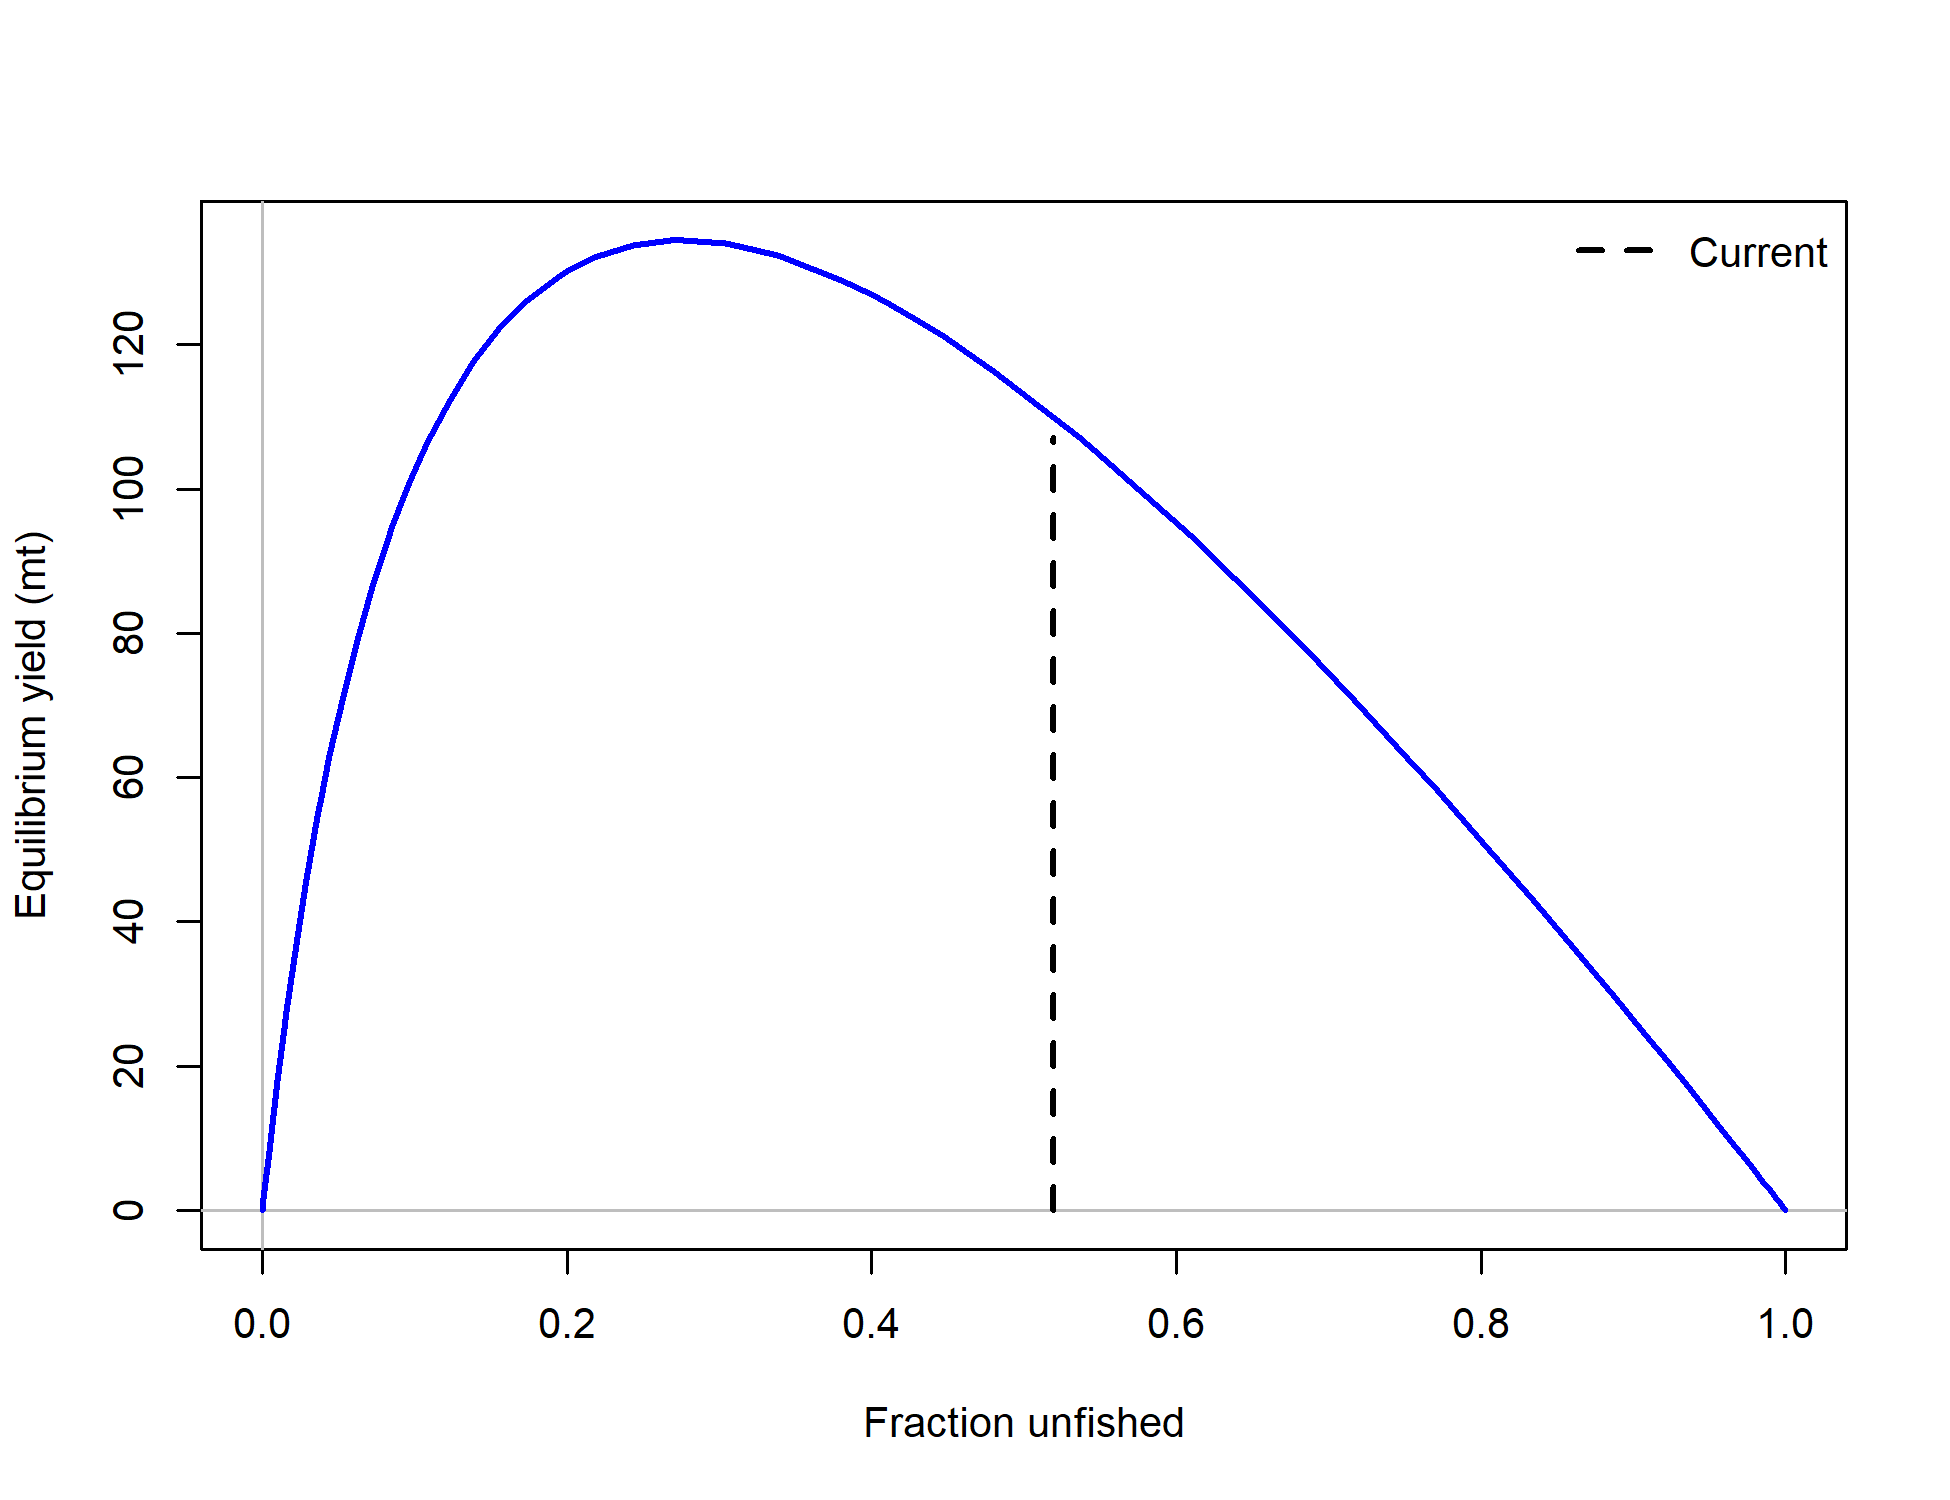
\includegraphics[width=1\textwidth,height=1\textheight]{N:/Assessments/CurrentAssessments/copper_rockfish_2023/models/sca/_bridging/2.4_dw/plots/yield2_yield_curve_with_refpoints.png}
\caption{Equilibrium yield curve for the base case model. Values are based on the 2020 fishery selectivities and with steepness fixed at 0.80.\label{fig:yield}}
\end{figure}

\hypertarget{appendix-a}{%
\section{Appendix A}\label{appendix-a}}

\hypertarget{detailed-fit-to-length-composition-data}{%
\subsection{Detailed Fit to Length Composition Data}\label{detailed-fit-to-length-composition-data}}

\hypertarget{detailed-fit-to-age-composition-data}{%
\subsection{Detailed Fit to Age Composition Data}\label{detailed-fit-to-age-composition-data}}

\hypertarget{detailed-fit-to-conditional-age-at-length-composition-data}{%
\subsection{Detailed Fit to Conditional-Age-at-Length Composition Data}\label{detailed-fit-to-conditional-age-at-length-composition-data}}

\hypertarget{appendix-b.-mrfss-dockside-index-of-abundance}{%
\section{Appendix B. MRFSS Dockside Index of Abundance}\label{appendix-b.-mrfss-dockside-index-of-abundance}}

\hypertarget{appendix-c.-california-onboard-cpfv-index-of-abundance}{%
\section{Appendix C. California Onboard CPFV Index of Abundance}\label{appendix-c.-california-onboard-cpfv-index-of-abundance}}

\hypertarget{appendix-d.-crfs-pr-dockside-index-of-abundance}{%
\section{Appendix D. CRFS PR Dockside Index of Abundance}\label{appendix-d.-crfs-pr-dockside-index-of-abundance}}

\hypertarget{appendix-e.-ccfrp-index-of-abundance}{%
\section{Appendix E. CCFRP Index of Abundance}\label{appendix-e.-ccfrp-index-of-abundance}}

\hypertarget{appendix-f.-nwfsc-hook-and-line-index-of-abundance}{%
\section{Appendix F. NWFSC Hook and Line Index of Abundance}\label{appendix-f.-nwfsc-hook-and-line-index-of-abundance}}

Since 2004, the NWFSC has conducted an annual hook and line survey targeting shelf rockfish in the genus \emph{Sebastes} at fixed stations (e.g., sites, Figure \ref{fig:nwfsc-hkl-map}) in the Southern California Bight. Key species of rockfish targeted by the NWFSC Hook and Line survey are bocaccio (\emph{S. paucispinis}), cowcod (\emph{S. levis}), greenspotted (\emph{S. chlorostictus}), and vermilion/sunset (\emph{S. miniatus} and \emph{S. crocotulus}) rockfishes, although a wide range of rockfish species have been observed by this survey. During each site visit, three deckhands simultaneously deploy 5-hook sampling rigs (this is referred to as a single drop) for a maximum of 5 minutes per line, but individual lines may be retrieved sooner at the angler's discretion (e.g., to avoid losing fish). Five drops are attempted at each site for a maximum possible catch of 75 fish per site per year (3 anglers x 5 hooks x 5 drops). Further details regarding the sample frame, site selection, and survey methodology are described by Harms et al. (2008).

The sites considered for the creation of a relative index of abundance were limited to sites that have caught at least 1 copper rockfish across all years. A range of alternative model structures were explored to generate an index of abundances. This included alternative levels of aggregation (hook, drop, or site), probability distributions (negative binomial, delta-gamma, or delta-lognormal), and covariates (year, site number, depth, swell height, inside/outside CCA, and/or the number of vermilion/sunset or bocaccio rockfishes observed, Table ref\{tab:nwfsc-hkl-model-selection\}). The overall trend in the index of abundance were highly similar across the explored probability distributions and model configurations. The number of observation in copper rockfish in the CCA were limited. The calculated CPUE inside and outside the CCA were similar for copper rockfish (Figure \ref{fig:nwfsc-hkl-cca}). Given this, the index selected for the base model include all observations of copper rockfish across all sampled sites. Sensitivities to excluding the CCA observations were conducted.

All modeling was initially conducted using sdmTMB (Anderson et al. 2022) with the final selected model fit using the ``rstanarm'' R package (v. 2.21.3). All diagnostics appearred reasonable. The final selected model was a negative binomial model that included covariates terms for year, site number, drop, swell height, and the number of bocaccio and vermilion/sunset rockfishes separately. A comparison between the standardized estimated relative index of abundance compared with the calculated raw catch-per-unit-effort (CPUE) is show Figure \ref{fig:nwfsc-hkl-index-raw}. The final index of abundance is shown in Figure \ref{fig:nwfsc-hkl-index} and Table \ref{tab:nwfsc-hkl-index}

\pagebreak

\begingroup\fontsize{10}{12}\selectfont
\begingroup\fontsize{10}{12}\selectfont

\begin{longtable}[t]{r>{\centering\arraybackslash}p{1cm}>{\centering\arraybackslash}p{1cm}>{\centering\arraybackslash}p{1cm}>{\centering\arraybackslash}p{1cm}>{\centering\arraybackslash}p{1cm}>{\centering\arraybackslash}p{1cm}>{\centering\arraybackslash}p{1cm}>{\centering\arraybackslash}p{1cm}>{\centering\arraybackslash}p{1cm}>{\centering\arraybackslash}p{1cm}}
\caption{\label{tab:nwfsc-hkl-model-select}Model selection for the NWFSC Hook and Line survey.}\\
\toprule
Bocaccio & Drop & Moon & Site & Swell & Vermilion & Year & Offset-log(effort) & DF & AICc & Delta\\
\midrule
\endfirsthead
\caption[]{Model selection for the NWFSC Hook and Line survey. \textit{(continued)}}\\
\toprule
Bocaccio & Drop & Moon & Site & Swell & Vermilion & Year & Offset-log(effort) & DF & AICc & Delta\\
\midrule
\endhead

\endfoot
\bottomrule
\endlastfoot
-0.03 & + & NA & + & -0.42 & 0.05 & + & + & 97 & 5113.3 & 0.0\\
NA & + & NA & + & -0.43 & 0.05 & + & + & 96 & 5113.3 & 0.1\\
-0.03 & + & 0 & + & -0.41 & 0.05 & + & + & 98 & 5114.3 & 1.0\\
NA & + & 0 & + & -0.41 & 0.05 & + & + & 97 & 5114.4 & 1.2\\
-0.03 & + & NA & + & -0.45 & NA & + & + & 96 & 5123.0 & 9.8\\
NA & + & NA & + & -0.45 & NA & + & + & 95 & 5123.1 & 9.9\\
-0.03 & + & NA & + & NA & 0.05 & + & + & 96 & 5123.5 & 10.3\\
-0.03 & + & 0 & + & NA & 0.05 & + & + & 97 & 5123.6 & 10.4\\
NA & + & NA & + & NA & 0.05 & + & + & 95 & 5123.7 & 10.5\\
NA & + & 0 & + & NA & 0.05 & + & + & 96 & 5123.9 & 10.6\\
-0.03 & + & 0 & + & -0.44 & NA & + & + & 97 & 5124.2 & 11.0\\
NA & + & 0 & + & -0.44 & NA & + & + & 96 & 5124.4 & 11.1\\
-0.03 & + & NA & + & NA & NA & + & + & 95 & 5134.6 & 21.4\\
NA & + & NA & + & NA & NA & + & + & 94 & 5134.9 & 21.6\\
-0.03 & + & 0 & + & NA & NA & + & + & 96 & 5134.9 & 21.6\\
NA & + & 0 & + & NA & NA & + & + & 95 & 5135.2 & 21.9\\*
\end{longtable}
\endgroup{}
\endgroup{}


\begin{figure}
\centering
\includegraphics[width=1\textwidth,height=1\textheight]{N:/Assessments/CurrentAssessments/copper_rockfish_2023/data/nwfsc_hkl/plots/standardized_cpue_nwfsc_hkl_inside_outside.png}
\caption{Standardized CPUE inside and outside the CCA.\label{fig:nwfsc-hkl-cca}}
\end{figure}

\newpage

\begin{figure}
\centering
\includegraphics[width=1\textwidth,height=1\textheight]{N:/Assessments/CurrentAssessments/copper_rockfish_2023/data/survey_indices/nwfsc_hkl/plots/stand_index_raw_versus_est.png}
\caption{Standardized comparison of estimated relative index of abundance and the raw cath-per-unit-effort.\label{fig:nwfsc-hkl-index-raw}}
\end{figure}

\newpage

\begin{figure}
\centering
\includegraphics[width=1\textwidth,height=1\textheight]{N:/Assessments/CurrentAssessments/copper_rockfish_2023/data/survey_indices/nwfsc_hkl/rstan_full_nb_glm_year_site_drop_swell_bocaccio_vermilon/Index.png}
\caption{Estimated index of abundance for copper rockfish.\label{fig:nwfsc-hkl-indices}}
\end{figure}

\hypertarget{appendix-g.-cdfw-rov-index-of-abundance}{%
\section{Appendix G. CDFW ROV Index of Abundance}\label{appendix-g.-cdfw-rov-index-of-abundance}}

The California Department of Fish and Wildlife (CDFW) in collaboration with Marine Applied Research and Exploration (MARE) have been conducting remotely operated vehicle (ROV) surveys along the California coast in Marine Protected Areas (MPAs) and reference sites adjacent to them since 2004 for the purposes of long-term monitoring of changes in size, density (fish/square meter) and length of fish and invertebrate species along the California coast. Surveys of the entire coast have now been undertaken twice, each taking three years to complete, 2014-2016 and again in 2019-2021. The survey conducted multiple 500 meter transects across rocky reef survey sites. Sample sites were selected by first randomly selecting the deepest transect at a given site, then selecting transects on a constant interval into shallower depths. Transects were designed to be oriented parallel to general depth contours, though they were carried out using a fixed bearing that crossed depths in some cases.

Given that each pass of the California coast took a three year period, the STAT opted to explore using the data with super years. The selected super years were 2015 and 2020. Given the life history of copper rockfish an the limited movement of adult copper rockfish especially given the range of the survey area each year, the super year application was deemed reasonable in order to consider these data within the model. Minimal filtering were done to the data. Transects were removed based on four factors: 1) extreme estimates of effort (the estimated area of view below the ROV termed usable area), 2) any locations that were not sampled by both super year periods, 3) transect that were conducted across MPA and reference areas, and 4) transect conducted across depths that never observed copper rockfish within the survey (Table \ref{tab:rov-filtered}). Once the data were filtered the average calculated CPUE for each MPA and Reference groups were plotted to visualize the data (Table \ref{tab:rov-obs} and Figure \ref{fig:rov-raw-cpue}).

A range of alternative model structures were explored to generate an index of abundances including alternative error structures, covariates, and factors were considered when exploring how best to model these data. Based on model selection a model with super year, site designation (MPA or Reference), proportion soft terrain, and super year site designation interaction was selected (Table \ref{tab:rov-model-selection}). A delta-lognormal model was selected based on the distribution of the data and diagnostics (Figure \ref{fig:rov-qq}) using sdmTMB (Anderson et al. 2022). The model estimates were then area-weighted based on the estimated percent of habitat within MPAs. An estimate of 8\% of rocky habitat within MPAs south of Point Conception and 92\% open to fishing were provided by John Budrick (CDFW). The estimated relative index of abundance is shown in Table \ref{tab:rov-index} and Figure \ref{fig:rov-index}.

\newpage

\begingroup\fontsize{10}{12}\selectfont
\begingroup\fontsize{10}{12}\selectfont

\begin{longtable}[t]{r>{\centering\arraybackslash}p{2cm}}
\caption{\label{tab:rov-filtered}Number of records filtered during data processing for the ROV survey data and the total remaining records.}\\
\toprule
Removal reason & Number\\
\midrule
\endfirsthead
\caption[]{Number of records filtered during data processing for the ROV survey data and the total remaining records. \textit{(continued)}}\\
\toprule
Removal reason & Number\\
\midrule
\endhead

\endfoot
\bottomrule
\endlastfoot
Records with usable area outside the 96th quantile & 36\\
Records with depths outside 19.3 - 99.8 m & 3\\
Transects that were both inside and outside MPA area & 41\\
Reference or MPA locations without sampling for at least three years & 12\\
Retained records & 798\\*
\end{longtable}
\endgroup{}
\endgroup{}


\newpage

\begingroup\fontsize{10}{12}\selectfont
\begingroup\fontsize{10}{12}\selectfont

\begin{longtable}[t]{r>{\centering\arraybackslash}p{2.2cm}>{\centering\arraybackslash}p{2.2cm}>{\centering\arraybackslash}p{2.2cm}>{\centering\arraybackslash}p{2.2cm}}
\caption{\label{tab:rov-obs}Number of transects and number of observations of copper rockfish for each group and survey year.}\\
\toprule
Designation & MPA Group & Super Year & Transects & Observations\\
\midrule
\endfirsthead
\caption[]{Number of transects and number of observations of copper rockfish for each group and survey year. \textit{(continued)}}\\
\toprule
Designation & MPA Group & Super Year & Transects & Observations\\
\midrule
\endhead

\endfoot
\bottomrule
\endlastfoot
MPA & Anacapa Island & 2015 & 48 & 139\\
MPA & Campus Point & 2015 & 4 & 2\\
Reference & Campus Point & 2015 & 6 & 0\\
MPA & Carrington Point & 2015 & 25 & 108\\
Reference & Carrington Point & 2015 & 23 & 190\\
MPA & Farnsworth & 2015 & 10 & 18\\
Reference & Farnsworth & 2015 & 14 & 11\\
MPA & Gull Island & 2015 & 42 & 404\\
Reference & Gull Island & 2015 & 36 & 66\\
MPA & Harris Point & 2015 & 27 & 244\\
Reference & Harris Point & 2015 & 18 & 40\\
MPA & Point Conception & 2015 & 8 & 13\\
Reference & Point Conception & 2015 & 4 & 0\\
MPA & South La Jolla & 2015 & 6 & 0\\
Reference & South La Jolla & 2015 & 13 & 1\\
MPA & South Point & 2015 & 24 & 179\\
Reference & South Point & 2015 & 22 & 50\\
MPA & Swami's & 2015 & 6 & 0\\
Reference & Swami's & 2015 & 14 & 0\\
MPA & Anacapa Island & 2020 & 30 & 58\\
MPA & Campus Point & 2020 & 21 & 27\\
Reference & Campus Point & 2020 & 8 & 2\\
MPA & Carrington Point & 2020 & 37 & 209\\
Reference & Carrington Point & 2020 & 24 & 139\\
MPA & Farnsworth & 2020 & 18 & 30\\
Reference & Farnsworth & 2020 & 25 & 7\\
MPA & Gull Island & 2020 & 34 & 198\\
Reference & Gull Island & 2020 & 31 & 82\\
MPA & Harris Point & 2020 & 30 & 438\\
Reference & Harris Point & 2020 & 15 & 58\\
MPA & Point Conception & 2020 & 13 & 72\\
Reference & Point Conception & 2020 & 6 & 5\\
MPA & South La Jolla & 2020 & 22 & 3\\
Reference & South La Jolla & 2020 & 24 & 4\\
MPA & South Point & 2020 & 30 & 218\\
Reference & South Point & 2020 & 25 & 70\\
MPA & Swami's & 2020 & 10 & 10\\
Reference & Swami's & 2020 & 15 & 1\\*
\end{longtable}
\endgroup{}
\endgroup{}


\newpage

\begingroup\fontsize{7}{9}\selectfont

\begin{landscape}\begingroup\fontsize{7}{9}\selectfont

\begin{longtable}[t]{l>{\raggedright\arraybackslash}p{0.92cm}>{\raggedright\arraybackslash}p{0.92cm}>{\raggedright\arraybackslash}p{0.92cm}>{\raggedright\arraybackslash}p{0.92cm}>{\raggedright\arraybackslash}p{0.92cm}>{\raggedright\arraybackslash}p{0.92cm}>{\raggedright\arraybackslash}p{0.92cm}>{\raggedright\arraybackslash}p{0.92cm}>{\raggedright\arraybackslash}p{0.92cm}>{\raggedright\arraybackslash}p{0.92cm}>{\raggedright\arraybackslash}p{0.92cm}}
\caption{\label{tab:rov-model-selection}Model selection for the ROV survey.}\\
\toprule
Designation & Depth.Polynomial & Prop..Hard & Prop..Mixed & Prop..Soft & Super.Year & Designation.Super\_year & offset.log.usable.area. & DF & log.likelihood & AICc & Delta\\
\midrule
\endfirsthead
\caption[]{\label{tab:rov-model-selection}Model selection for the ROV survey. \textit{(continued)}}\\
\toprule
Designation & Depth.Polynomial & Prop..Hard & Prop..Mixed & Prop..Soft & Super.Year & Designation.Super\_year & offset.log.usable.area. & DF & log.likelihood & AICc & Delta\\
\midrule
\endhead

\endfoot
\bottomrule
\endlastfoot
+ & + & N.A. & N.A. & -1.71 & + & NA & + & 7 & -1823.9 & 3661.8 & 0.00\\
+ & + & N.A. & N.A. & -1.71 & + & + & + & 8 & -1823.5 & 3663.2 & 1.39\\
+ & + & 1.76 & 1.64 & N.A. & + & NA & + & 8 & -1823.8 & 3663.8 & 1.95\\
+ & + & 0.12 & N.A. & -1.64 & + & NA & + & 8 & -1823.8 & 3663.8 & 1.95\\
+ & + & N.A. & -0.12 & -1.76 & + & NA & + & 8 & -1823.8 & 3663.8 & 1.95\\
+ & + & 101334179.47 & 101334179.37 & 101334177.71 & + & NA & + & 9 & -1823.3 & 3664.8 & 3.00\\
+ & + & 1.76 & 1.64 & N.A. & + & + & + & 9 & -1823.5 & 3665.2 & 3.36\\
+ & + & 0.12 & N.A. & -1.64 & + & + & + & 9 & -1823.5 & 3665.2 & 3.36\\
+ & + & N.A. & -0.12 & -1.76 & + & + & + & 9 & -1823.5 & 3665.2 & 3.36\\
+ & + & 99217437.47 & 99217437.37 & 99217435.71 & + & + & + & 10 & -1823.0 & 3666.3 & 4.45\\
+ & + & 1.5 & N.A. & N.A. & + & NA & + & 7 & -1836.2 & 3686.6 & 24.76\\
+ & + & 1.49 & N.A. & N.A. & + & + & + & 8 & -1835.9 & 3688.0 & 26.17\\
+ & + & N.A. & 1.26 & N.A. & + & NA & + & 7 & -1842.7 & 3699.5 & 37.64\\
+ & + & N.A. & 1.26 & N.A. & + & + & + & 8 & -1842.2 & 3700.6 & 38.79\\
+ & + & N.A. & N.A. & N.A. & + & NA & + & 6 & -1849.7 & 3711.5 & 49.66\\
+ & + & N.A. & N.A. & N.A. & + & + & + & 7 & -1849.3 & 3712.7 & 50.83\\
+ & NA & N.A. & N.A. & -1.62 & + & NA & + & 5 & -1854.0 & 3718.1 & 56.27\\
+ & NA & N.A. & N.A. & -1.62 & + & + & + & 6 & -1853.6 & 3719.3 & 57.47\\
+ & NA & 1.7 & 1.5 & N.A. & + & NA & + & 6 & -1853.9 & 3719.9 & 58.09\\
+ & NA & 0.2 & N.A. & -1.5 & + & NA & + & 6 & -1853.9 & 3719.9 & 58.09\\
+ & NA & N.A. & -0.2 & -1.7 & + & NA & + & 6 & -1853.9 & 3719.9 & 58.09\\
+ & NA & 102962691.18 & 102962691 & 102962689.48 & + & NA & + & 7 & -1853.4 & 3721.0 & 59.15\\
+ & NA & 1.7 & 1.51 & N.A. & + & + & + & 7 & -1853.5 & 3721.2 & 59.31\\
+ & NA & 0.19 & N.A. & -1.51 & + & + & + & 7 & -1853.5 & 3721.2 & 59.31\\
+ & NA & N.A. & -0.19 & -1.7 & + & + & + & 7 & -1853.5 & 3721.2 & 59.31\\
+ & NA & 100001585.01 & 100001584.84 & 100001583.31 & + & + & + & 8 & -1853.0 & 3722.3 & 60.44\\
+ & NA & 1.76 & N.A. & N.A. & + & NA & + & 5 & -1865.4 & 3740.8 & 79.00\\
+ & NA & 1.76 & N.A. & N.A. & + & + & + & 6 & -1865.1 & 3742.3 & 80.49\\
+ & NA & N.A. & 1.55 & N.A. & + & NA & + & 5 & -1874.9 & 3759.8 & 98.00\\
+ & NA & N.A. & 1.55 & N.A. & + & + & + & 6 & -1874.5 & 3761.1 & 99.30\\
+ & NA & N.A. & N.A. & N.A. & + & NA & + & 4 & -1885.8 & 3779.7 & 117.89\\
+ & NA & N.A. & N.A. & N.A. & + & + & + & 5 & -1885.6 & 3781.2 & 119.35\\*
\end{longtable}
\endgroup{}
\end{landscape}
\endgroup{}

\newpage

\begingroup\fontsize{10}{12}\selectfont
\begingroup\fontsize{10}{12}\selectfont

\begin{longtable}[t]{c>{\centering\arraybackslash}p{2cm}>{\centering\arraybackslash}p{2cm}}
\caption{\label{tab:rov-index}Estimated relative index of abundance for the ROV survey.}\\
\toprule
Year & Estimate & logSE\\
\midrule
\endfirsthead
\caption[]{\label{tab:rov-index}Estimated relative index of abundance for the ROV survey. \textit{(continued)}}\\
\toprule
Year & Estimate & logSE\\
\midrule
\endhead

\endfoot
\bottomrule
\endlastfoot
2015 & 0.2044865 & 0.1373854\\
2020 & 0.1981717 & 0.1261661\\*
\end{longtable}
\endgroup{}
\endgroup{}

\newpage

\begin{figure}
\centering
\includegraphics[width=1\textwidth,height=1\textheight]{N:/Assessments/CurrentAssessments/copper_rockfish_2023/data/survey_indices/rov/plots/south_raw_cpue_by_mpa_group.png}
\caption{The trend of the calculated CPUE by each MPA and Reference group.\label{fig:rov-raw-cpue}}
\end{figure}

\newpage

\begin{figure}
\centering
\includegraphics[width=1\textwidth,height=1\textheight]{N:/Assessments/CurrentAssessments/copper_rockfish_2023/data/survey_indices/rov/delta_lognormal_south_designation_depth_soft/qq.png}
\caption{QQ-plot for the ROV survey.\label{fig:rov-qq}}
\end{figure}

\newpage

\begin{figure}
\centering
\includegraphics[width=1\textwidth,height=1\textheight]{N:/Assessments/CurrentAssessments/copper_rockfish_2023/data/survey_indices/rov/delta_lognormal_south_designation_depth_soft/Index.png}
\caption{The weighted relative index of abundance.\label{fig:rov-index}}
\end{figure}
\end{document}
